\tableofcontents

\section{Controlling the interparticle interactions in a correlated electron system}

Studying the interparticle interactions in a correlated electron system by applying laser pulses is a challenging perspective, which may lead to some states of matter that do not exist in equilibrium. For example, changing the electron-electron interaction from the original Coulomb repulsion to an attraction, can induce an s-wave superconducting state with very high transition temperature,1,2 or the BCS-BEC crossover.2,3

Creation a population inversion in metallic bands corresponding to a negative temperature (T) state.9,10 is one of the way to control the interaction. Such investigation done in work of \citet{PhysRevB.85.155124} for hipercubic lattice, where was shown that it is possible to induce a population inversion in metallic systems using a properly shaped  half-cycle or monocycle pulses, the system without energy dissipation will thermalize in the negative T state after the pulse. This implies an effective switching of the interaction from repulsive to attractive, since a density matrix $\exp(-H/T)$ for a Hamiltonian $H$ with temperature $T < 0$ corresponds to the one for the inverted $-H$ with $-T > 0$.11,12 

Effective switching of the interaction from repulsive to attractive occur because a density matrix $\exp({-H/T})$ for a Hamiltonian $H$ with temperature $T < 0$ corresponds inverted $-H$ with $-T > 0$.

%\clearpage
\subsection{Creation of population inversion by linear polarized electric field}


In this chapter we repeat work \citet{PhysRevB.85.155124} taking realistic 2d square lattice and focused in transient nonequilibrium dynamics with different polarization of electric field.
By the half-cycle pulse we induce shift in the momentum distribution of the electrons. Selecting the parameters of such a pulse we can achieve half of the Brillouin zone, the system is brought to a negative-T state, this is often (depending on the value of the interaction) leads to change of the interaction from repulsive to attractive.

\subsubsection{Half-cycle vector potential}


To investigate effects of negative temperature state we use single-band Hubbard model driven by an half-cycle electric field. Half-cycle pulse chosen in Y and diagonal directions to look polarisation dependence and iverson of population.

The vector potential has the form:

\begin{equation}
A(t)=\frac{A_{max}}{\tau}(t-\tau sin(2\pi t/\tau))
\end{equation}

where $A_{max}$ - amplitude of vector potential; $\tau$ - pulse length.

\begin{figure}[h!]
\begin{minipage}[h]{0.5\linewidth}
\center{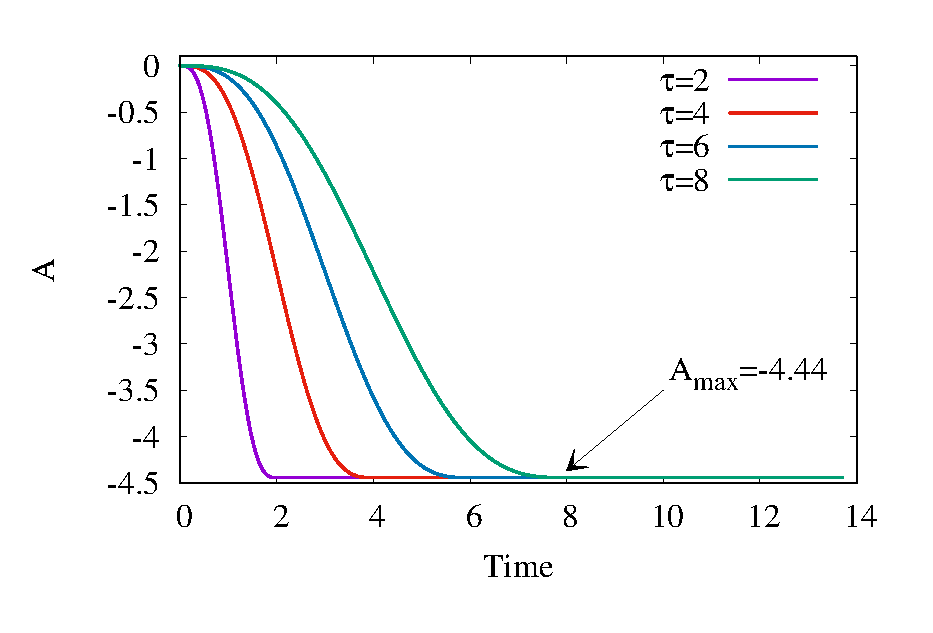
\includegraphics[width=1\linewidth]{figure/xy/PulseA.eps}} (a) \\
\end{minipage}
\hfill
\begin{minipage}[h]{0.5\linewidth}
\center{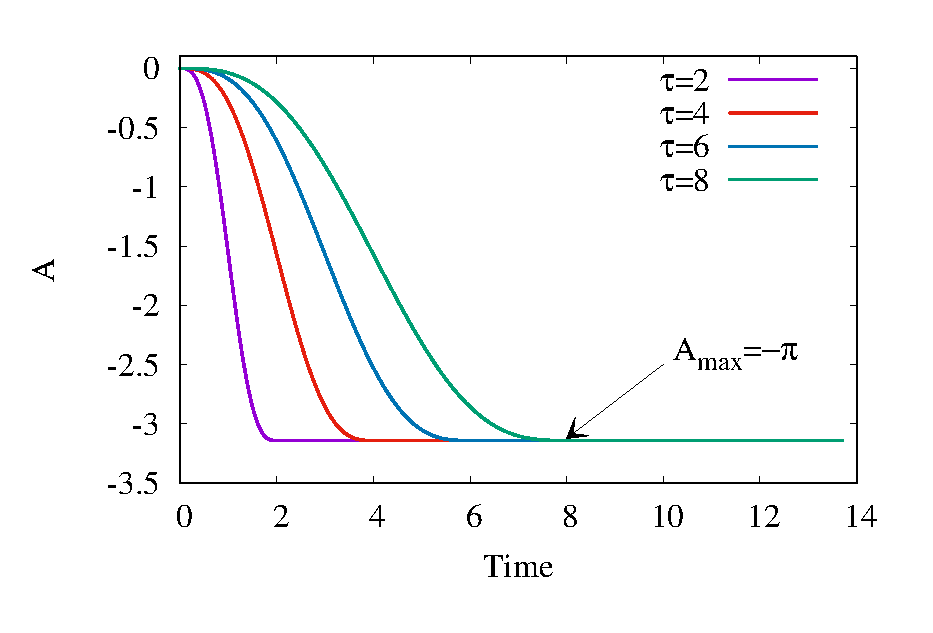
\includegraphics[width=1\linewidth]{figure/y/PulseA.eps}} \\(b)
\end{minipage}

\begin{minipage}[h]{0.5\linewidth}
\center{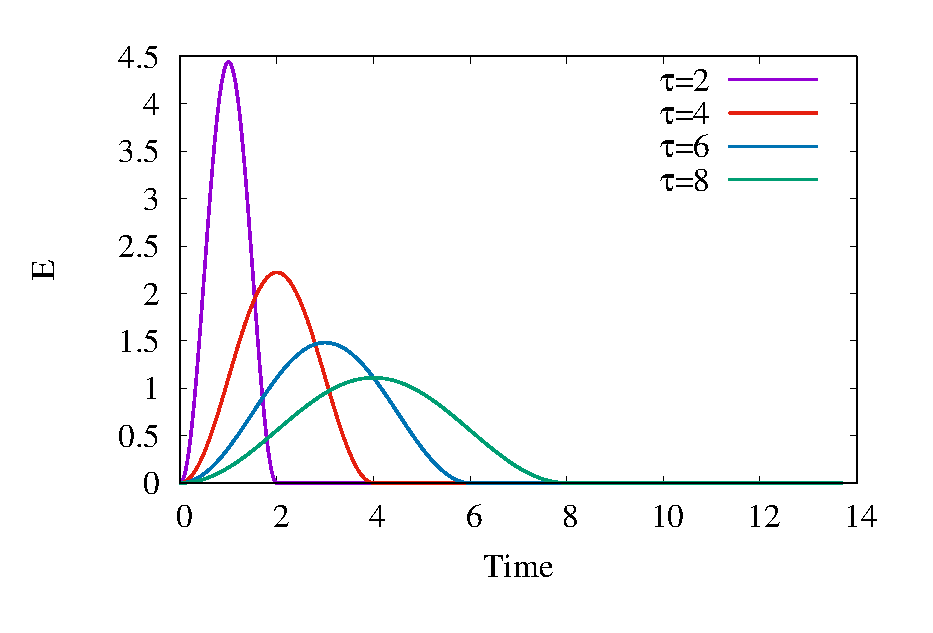
\includegraphics[width=1\linewidth]{figure/xy/PulseE.eps}} (c) \\
\end{minipage}
\hfill
\begin{minipage}[h]{0.5\linewidth}
\center{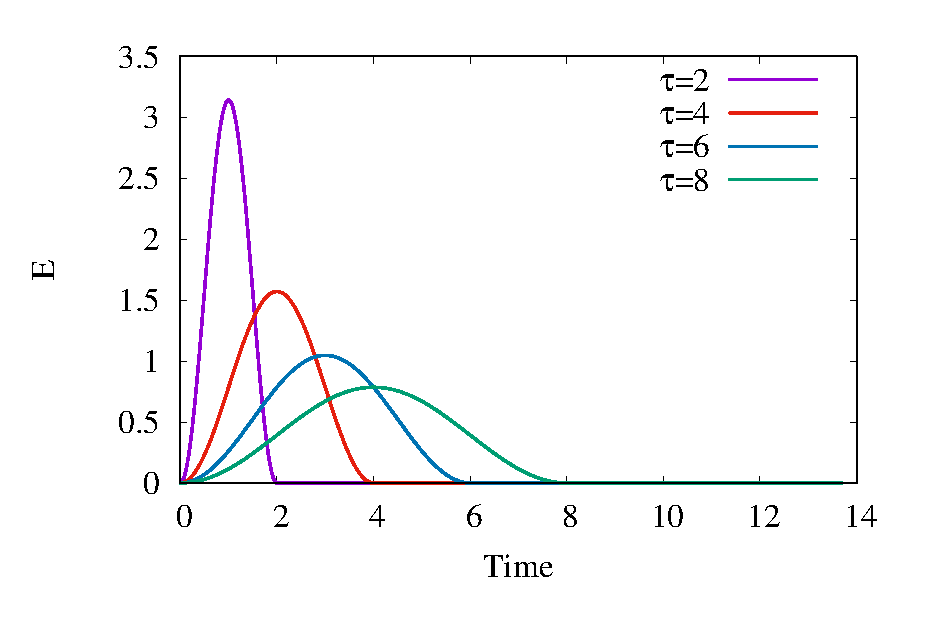
\includegraphics[width=1\linewidth]{figure/y/PulseE.eps}} \\(d)
\end{minipage}

\caption{Vector potential and external electric field: a,c for diagonal direction; b,d for Y direction}
\label{fig:Pulses}
\end{figure}


In case Y direction of field, the maximum value of the vector potential $A_{max} = \pi$ (Figure \ref{fig:Pulses}a,c). For diagonal direction of field the maximum value of the vector potential $A_{max} =\pi*\sqrt{2}$ (Figure \ref{fig:Pulses}b,d). This allows to shift the momentum distribution in the case of Y-field from $\Gamma$ to Y, in the case of diagonal field from $\Gamma$ to M in the Brillouin zone.

%\clearpage

\subsubsection{Total energy and double occupancy.}

From the total energy we can recognize the repulsion-to-attraction transition. After the pulse excitation isolated system is supposed to approach a thermalized state [25] with some effective temperature $T_{eff}$ and a total energy $E_{tot}$. A thermal state with a positive temperature has $E_{tot} < 0$ for the interaction term of the Hamiltonian at half filling, while $E_{tot} > 0$ happens at negative temperature. Thereby the total energy is an order parameter for the repulsion-to-attraction transition. Suchwise if $E_{tot} > 0$ the system arrives at a negative temperature state ($T_{eff} < 0$) \citet{PhysRevB.85.155124}.

To show effect of inversion population we choose half-cycle shape of electric field with $\tau = 4$ (red line in Figures \ref{fig:Pulses}c,d) and investigate behaviour of total energy and double occupancy (Figure \ref{fig:E_tot}).

\begin{figure}[h!]
\begin{minipage}[h]{0.5\linewidth}
\center{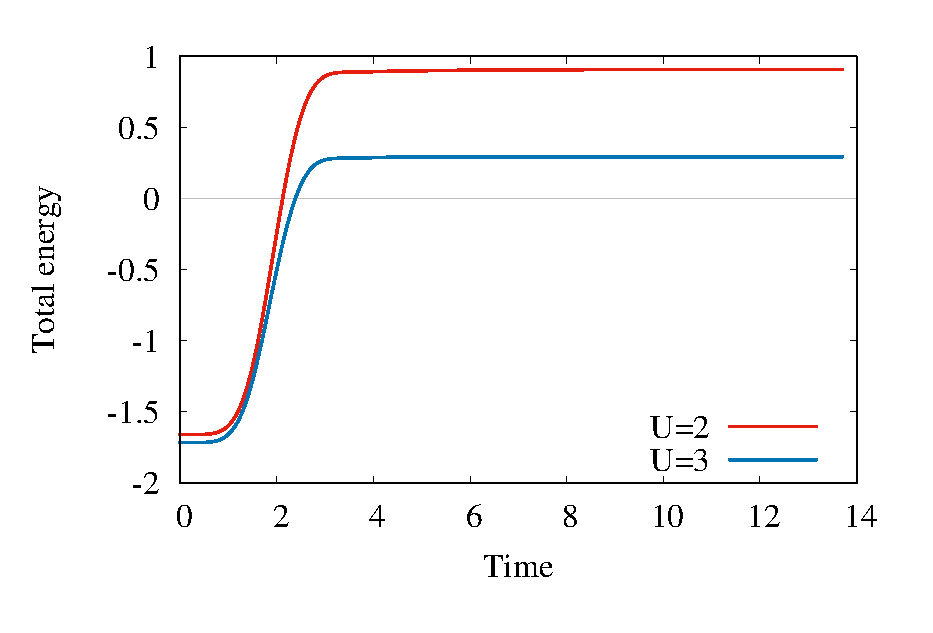
\includegraphics[width=1\linewidth]{figure/xy/E_tot_xy.eps}} (a) \\
\end{minipage}
\hfill
\begin{minipage}[h]{0.5\linewidth}
\center{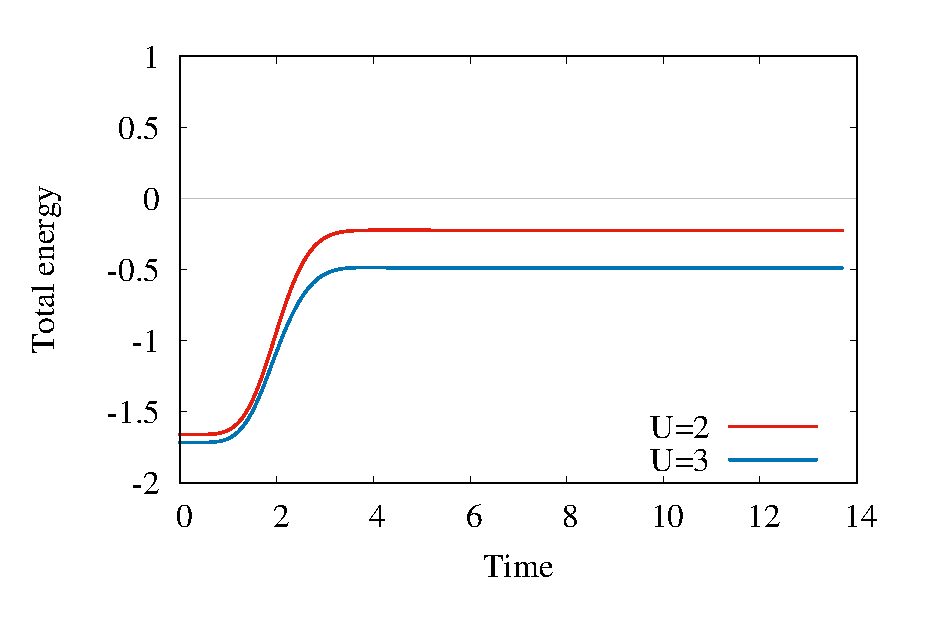
\includegraphics[width=1\linewidth]{figure/y/E_tot_y.eps}} \\(b)
\end{minipage}

\begin{minipage}[h]{0.5\linewidth}
\center{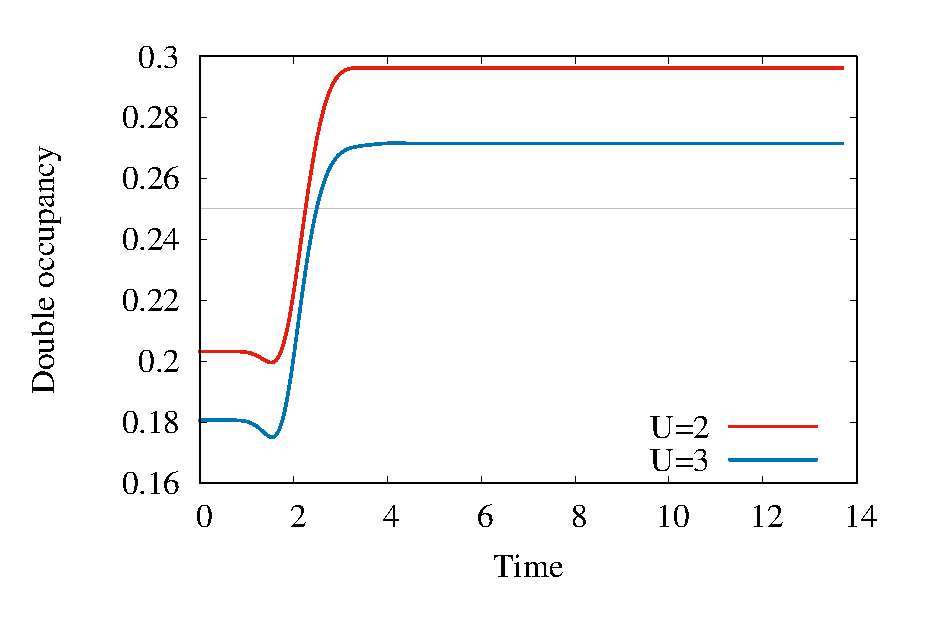
\includegraphics[width=1\linewidth]{figure/xy/docc_xy.eps}} (c) \\
\end{minipage}
\hfill
\begin{minipage}[h]{0.5\linewidth}
\center{\includegraphics[width=1\linewidth]{figure/y/docc_y.eps}} \\(d)
\end{minipage}

\caption{Total energy and double occupancy ($\tau = 4$): a,c for XY direction of pulse ($A_{max} =\pi\sqrt{2}$); b,d for Y direction of pulse ($A_{max} = \pi$).}
\label{fig:E_tot}
\end{figure}

From analysis of Fig. \ref{fig:E_tot} we can observe a change in the sign of the interaction in case of field in the diagonal direction, U=2 and U=3. $E_{tot}>0$ (the total energy has the origin at zero) and double occupancy $docc>0.25$ after the pulse. It seen then lower Coulomb interaction than $E_{tot}$ has bigger value and more pronounced effect of negative temperature state after pulse. In case of Y direction of electric field total energy negative all the time so the interaction does not change the sign. 


\begin{figure}[h!]
\center{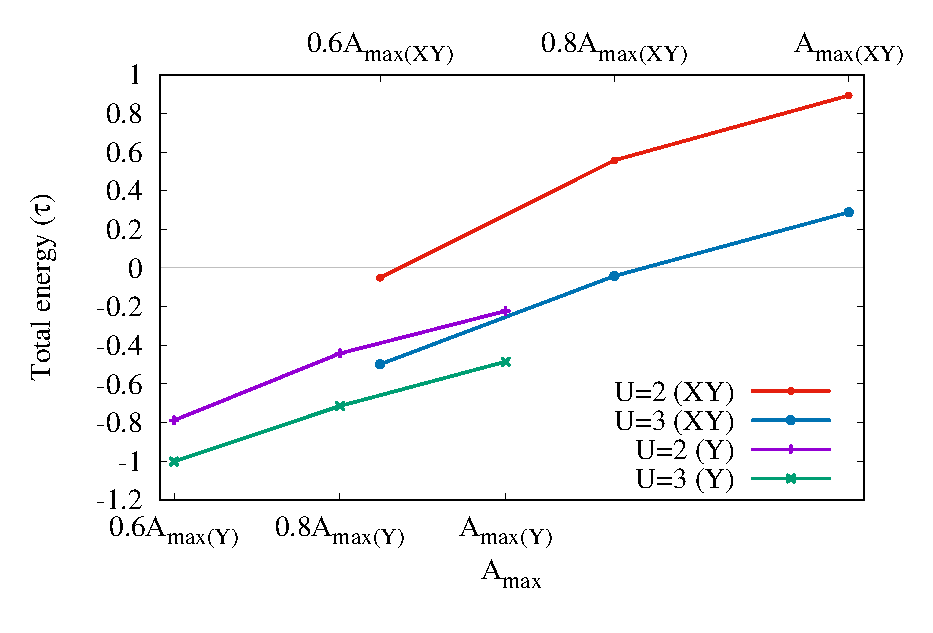
\includegraphics[width=0.7\linewidth]{figure/xy/E_mpi.eps}} \\
\caption{The total energy after the pulse as a function of the magnitude of the vector potential ($\tau = 4$).}
\label{fig:E_tot_A}
\end{figure}

In Figure \ref{fig:E_tot_A} is shown total energy after the pulse for $\tau=4$ as a function of the magnitude of the vector potential for diagonal and Y field directions. The graph shows that for the field in the diagonal direction there is a positive total energy which means that the sign of interaction has changed. The value of the total energy is maximum when the value of the amplitude of the vector potential such that exactly shift momentum distribution in the case of Y-field from $\Gamma$ to Y and in the case of diagonal field from $\Gamma$ to M in the Brillouin zone.
As the magnitude of the vector potential decreases, the total energy decreases and, for a certain value of the vector potential, the total energy becomes negative. This is in accordance with the results of article \citet{PhysRevB.85.155124}. When the interaction increased, the value of the total energy decreases and the range of values of the total energy for the different amplitudes of the vector potential. In Y-direction of the field, there is no change in the sign of the interaction with different values of the vector potential and the Coulomb interaction (U=2,3).


\begin{figure}[h!]
\center{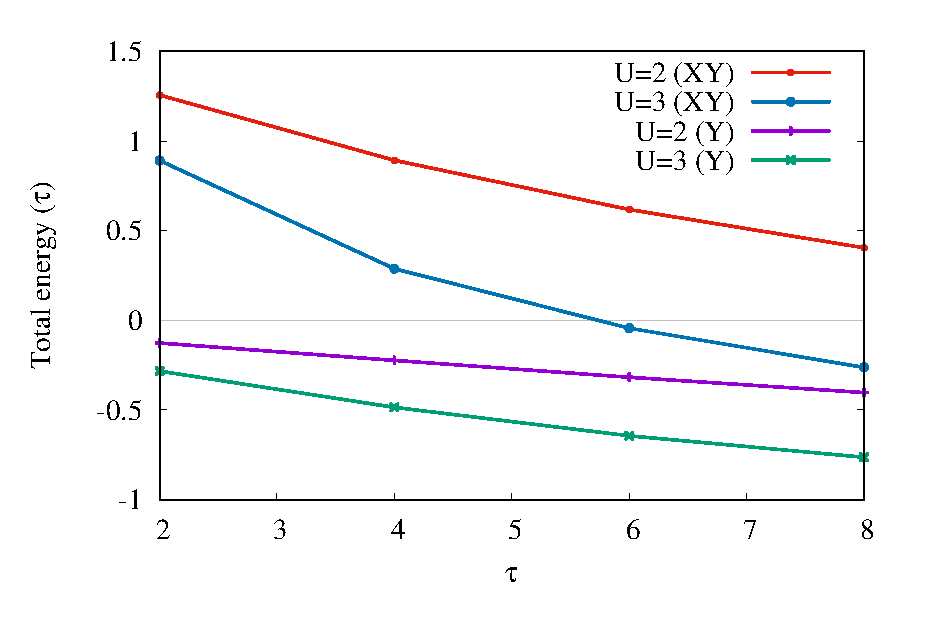
\includegraphics[width=0.7\linewidth]{figure/xy/E_tau.eps}} \\
\caption{The total energy after the pulse as a function of the pulse width.}
\label{fig:E_tot_tau}
\end{figure}
%\clearpage

The total energy after the pulse ($A_{max} = \pi$ Y-field; $A_{max} =\pi\sqrt{2}$ XY-field) as a function of pulse width depicted in Figure \ref{fig:E_tot_tau}. It can be seen from the figure that for a pulse with $\tau = 2$ (XY field direction), the total energy has a positive and maximum value (red and blue lines), this pulse narrowest in the calculations. With increasing pulse width, the total energy after the pulse can become negative, as seen on the blue line. This behavior was demonstrated also in the work [\citet{PhysRevB.85.155124}] for hypercubic lattice.
In the case of a pulse in the Y-direction, the total energy is always negative. With increasing pulse width the total energy goes to a more negative region.

\subsubsection{Momentum distribution. $A_{max}$-pulse.}

Visually change of electron population can be traced in time-dependent momentum distribution. This part shows the momentum distribution and how it varies with time under the action of half-cycle cosine pulse.

The Figure \ref{fig:md_u2_t0} shows momentum distribution of the interacting system (U=2) at time $t = 0$ when the system is in equilibrium and the field does not act on it. The maximum of the momentum distribution is at the $\Gamma$-point and the minimum at the angles of the first Brillouin zone.

\begin{figure}[h!]
\center{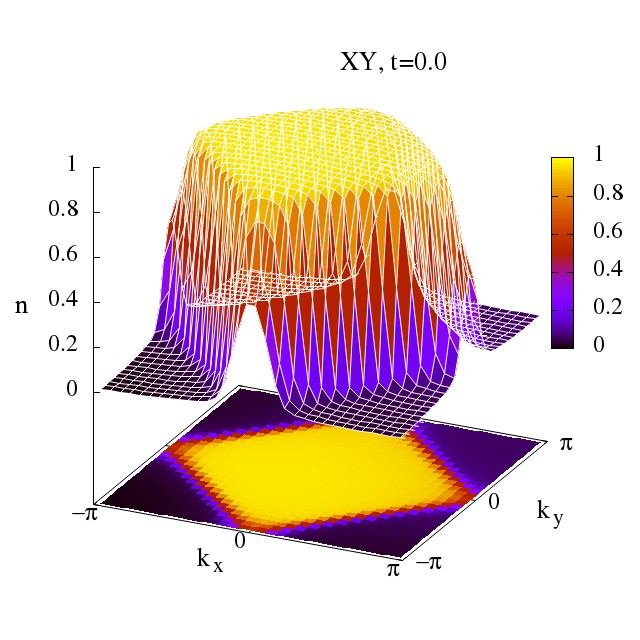
\includegraphics[width=0.6\linewidth]{figure/y/A_0.jpg}} \\
\caption{Equilibrium momentum distribution for U=2 at time=0.}
\label{fig:md_u2_t0}
\end{figure}

When the field is turned on, momentum distribution begins to move in the direction of the vector potential (or opposite to the direction of the electric field).

In Figure \ref{fig:md_u2_A_max} shown momentum distribution for U=2 during the action of the pulse. The pulse exists at time 0 to 4 ($\tau=4$). In the diagonal direction of the field (Figure \ref{fig:md_u2_A_max}a,c,e), the shift and flattening of the momentum distribution are seen. This shift leads to inversion of the population, since the maximum of the momentum distribution at the final instant of time (t=4) is at the corners of the first Brillouin zone and the minimum at the $\Gamma$-point. This finite distribution does not change much after the pulse (Figures \ref{fig:md_u2_A_max_relaxation}a,c,e). Also on (Figure \ref{fig:E_tot}a) seen that after the pulse the total energy is positive.

For a field in Y-direction there is no population inversion (Figures \ref{fig:md_u2_A_max}b,d,f). Under the influence of the field, it also shifts to the value of the vector potential. For the Y-direction momentum distribution has a long relaxation time (Figures \ref{fig:md_u2_A_max_relaxation}b,d,f) in comparison with the XY-direction (Figures \ref{fig:md_u2_A_max_relaxation}a,c,e).

\begin{figure}[h!]

\begin{minipage}[h]{0.43\linewidth}
\center{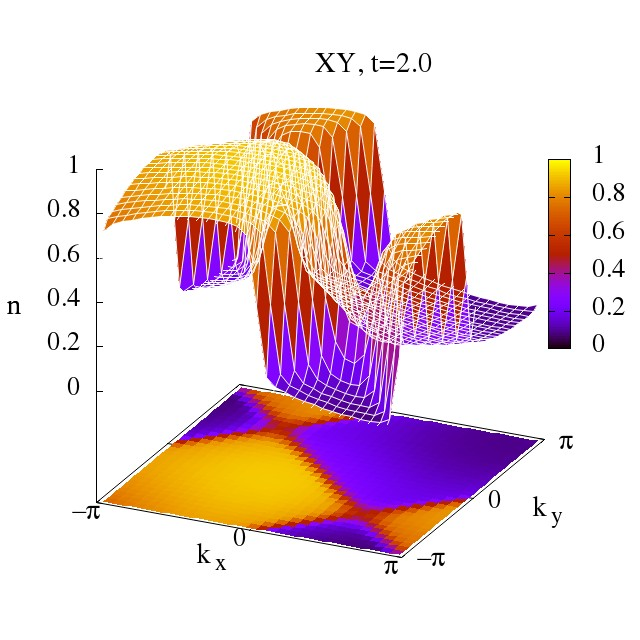
\includegraphics[width=1\linewidth]{figure/xy/u2/A_200.jpg}} (a) \\
\end{minipage}
\hfill
\begin{minipage}[h]{0.43\linewidth}
\center{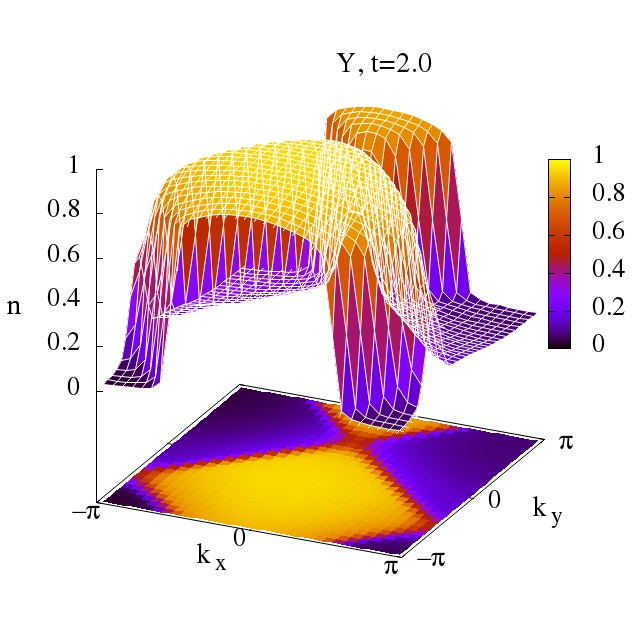
\includegraphics[width=1\linewidth]{figure/y/u2/A_200.jpg}} \\(b)
\end{minipage}
\begin{minipage}[h]{0.43\linewidth}
\center{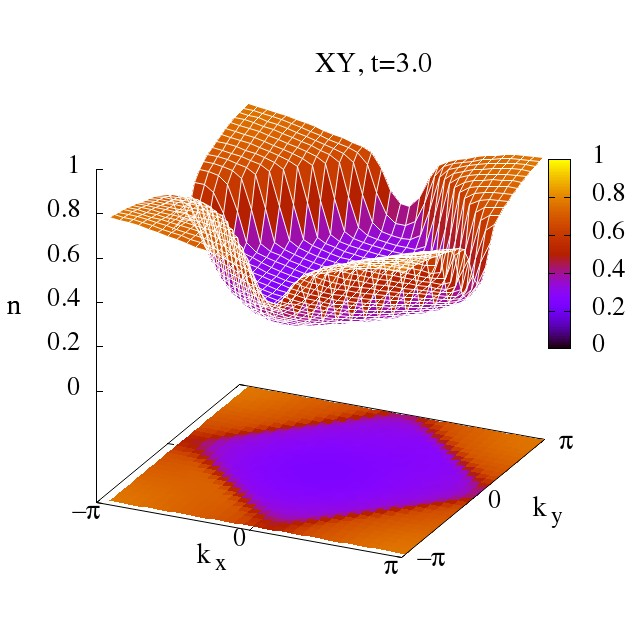
\includegraphics[width=1\linewidth]{figure/xy/u2/A_300.jpg}} (c) \\
\end{minipage}
\hfill
\begin{minipage}[h]{0.43\linewidth}
\center{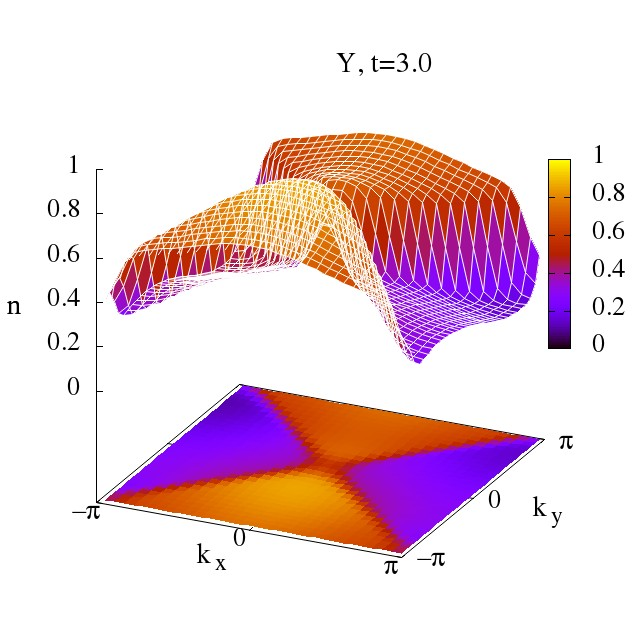
\includegraphics[width=1\linewidth]{figure/y/u2/A_300.jpg}} \\(d)
\end{minipage}
\begin{minipage}[h]{0.43\linewidth}
\center{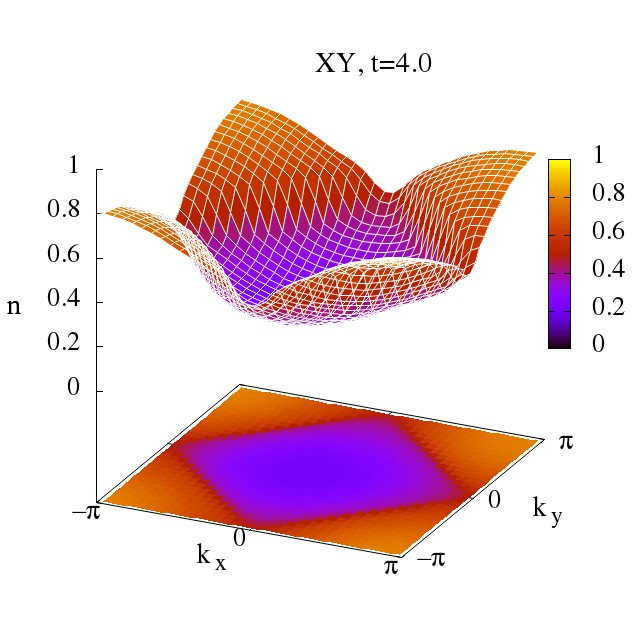
\includegraphics[width=1\linewidth]{figure/xy/u2/A_400.jpg}} (e) \\
\end{minipage}
\hfill
\begin{minipage}[h]{0.43\linewidth}
\center{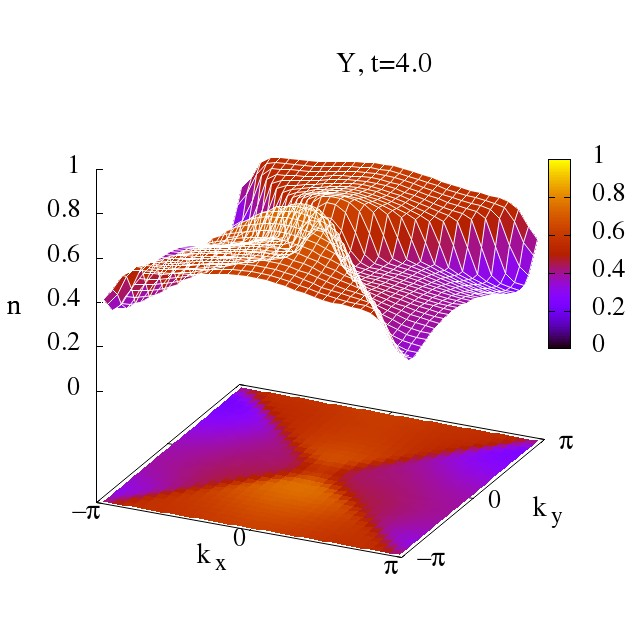
\includegraphics[width=1\linewidth]{figure/y/u2/A_400.jpg}} \\(f)
\end{minipage}
\caption{Momentum distribution for U=2 at different times (from 2 to 4), $\tau$=4. Left column a,c,e - field in XY direction; right column b,d,f - field in Y direction.}
\label{fig:md_u2_A_max}
\end{figure}
%\clearpage


\begin{figure}[h!]

\begin{minipage}[h]{0.43\linewidth}
\center{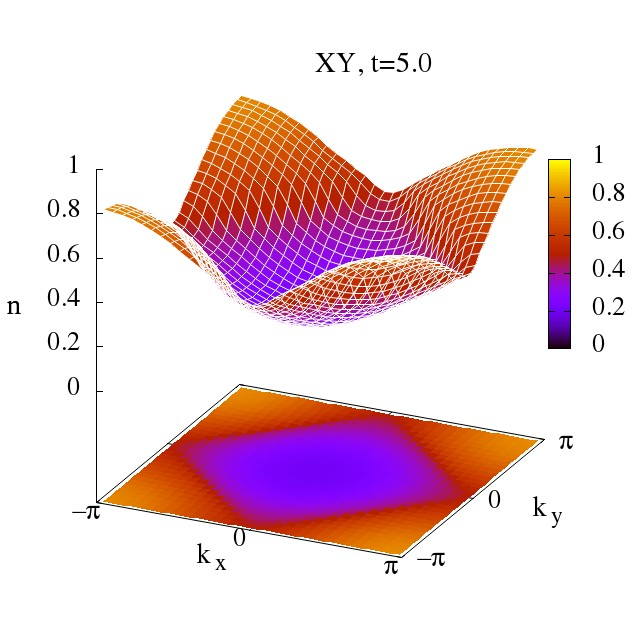
\includegraphics[width=1\linewidth]{figure/xy/u2/A_500.jpg}} (a) \\
\end{minipage}
\hfill
\begin{minipage}[h]{0.43\linewidth}
\center{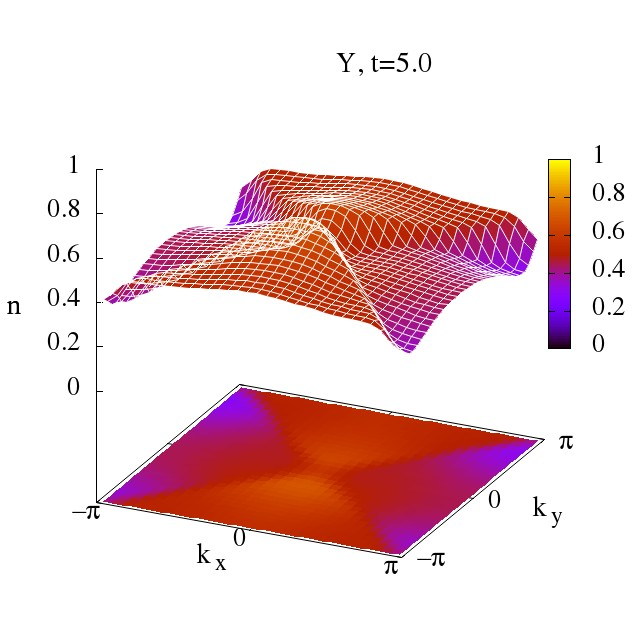
\includegraphics[width=1\linewidth]{figure/y/u2/A_500.jpg}} \\(b)
\end{minipage}
\begin{minipage}[h]{0.43\linewidth}
\center{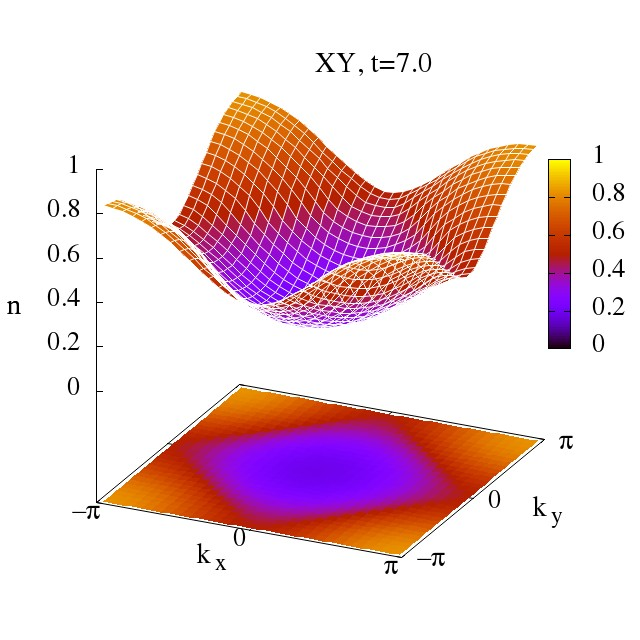
\includegraphics[width=1\linewidth]{figure/xy/u2/A_700.jpg}} (c) \\
\end{minipage}
\hfill
\begin{minipage}[h]{0.43\linewidth}
\center{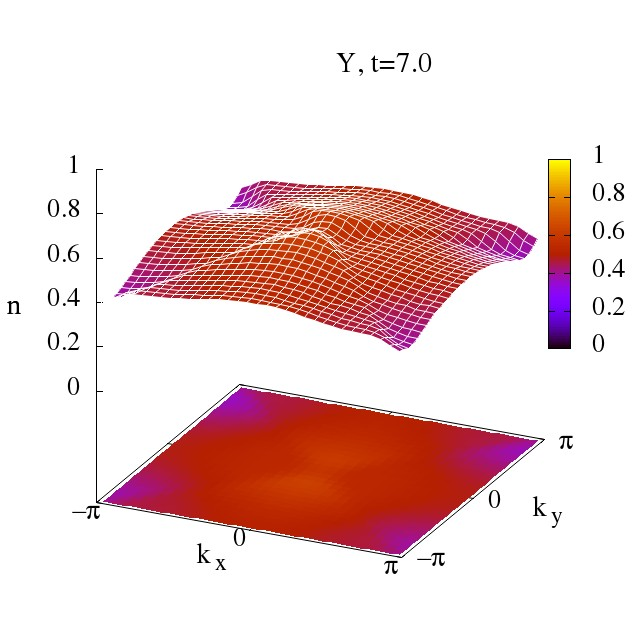
\includegraphics[width=1\linewidth]{figure/y/u2/A_700.jpg}} \\(d)
\end{minipage}
\begin{minipage}[h]{0.43\linewidth}
\center{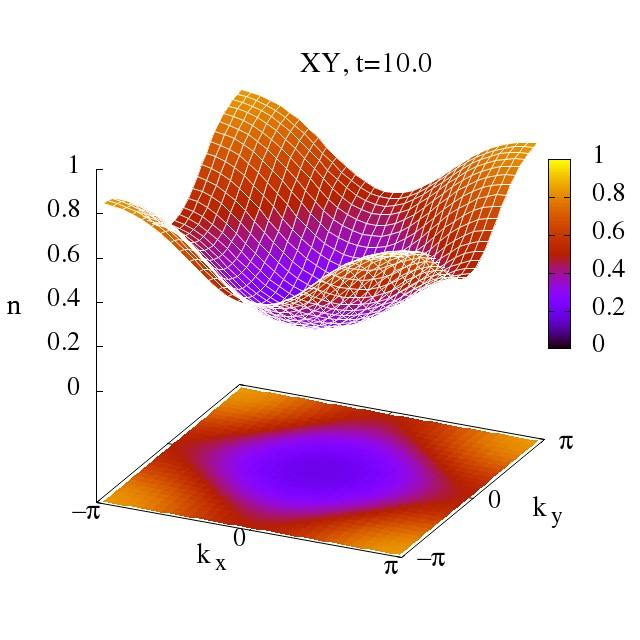
\includegraphics[width=1\linewidth]{figure/xy/u2/A_1000.jpg}} (e) \\
\end{minipage}
\hfill
\begin{minipage}[h]{0.43\linewidth}
\center{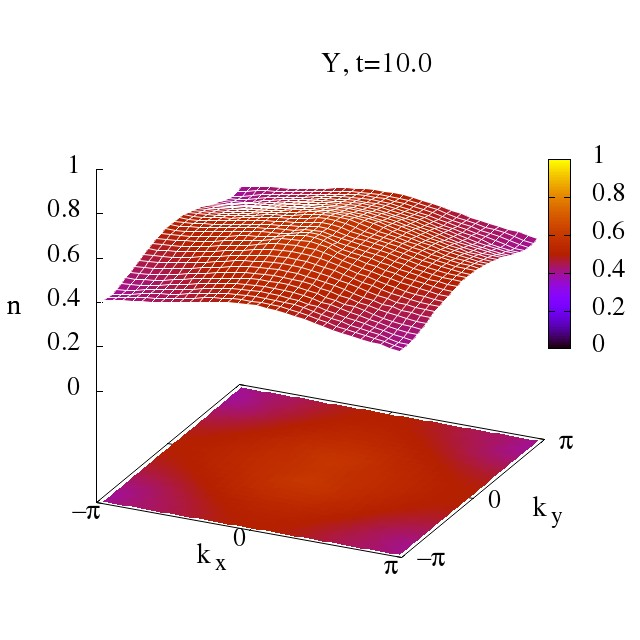
\includegraphics[width=1\linewidth]{figure/y/u2/A_1000.jpg}} \\(f)
\end{minipage}
\caption{Relaxation of momentum distribution (after pulse) for U=2 in different times (from 5 to 10), $\tau$=4. Left column a,c,e - field in XY direction; right column b,d,f - field in Y direction.}
\label{fig:md_u2_A_max_relaxation}
\end{figure}
%\clearpage


\begin{figure}[h!]
\begin{minipage}[h]{0.43\linewidth}
\center{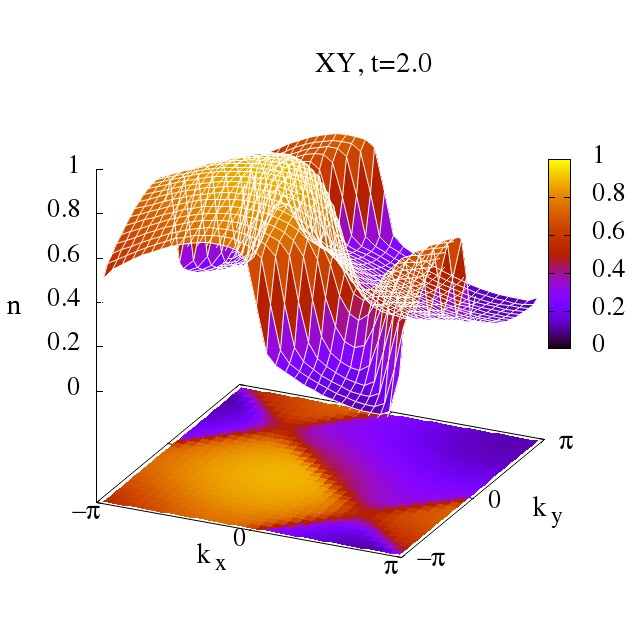
\includegraphics[width=1\linewidth]{figure/xy/u3/A_200.jpg}} (a) \\
\end{minipage}
\hfill
\begin{minipage}[h]{0.43\linewidth}
\center{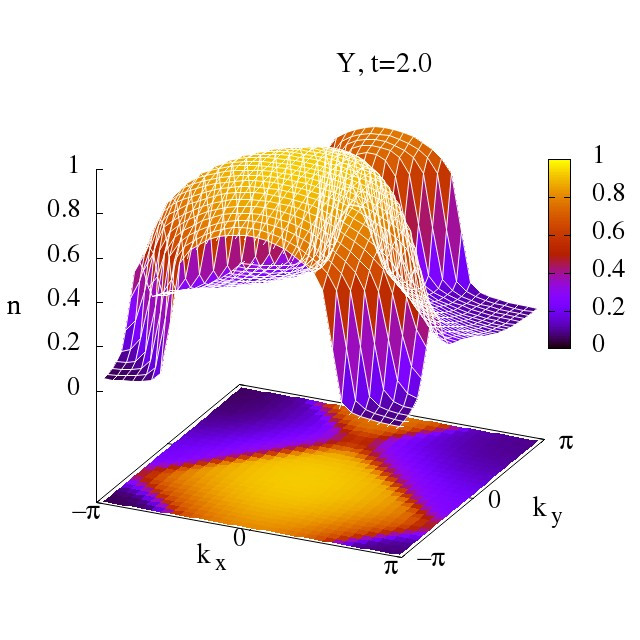
\includegraphics[width=1\linewidth]{figure/y/u3/A_200.jpg}} \\(b)
\end{minipage}
\begin{minipage}[h]{0.43\linewidth}
\center{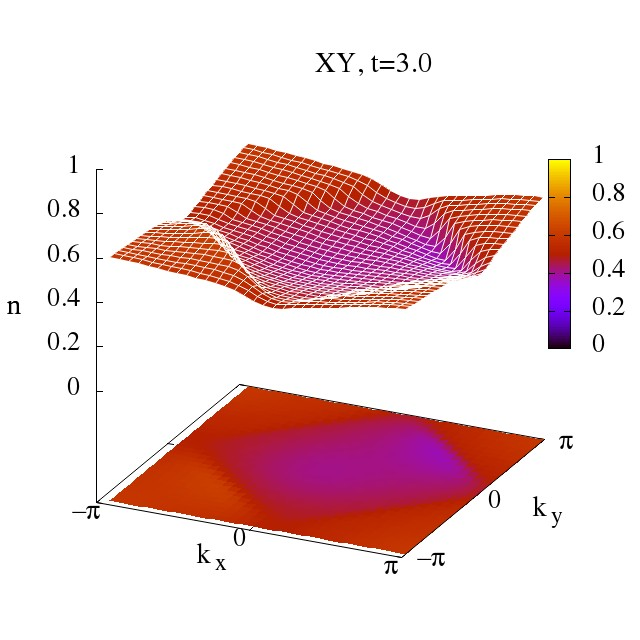
\includegraphics[width=1\linewidth]{figure/xy/u3/A_300.jpg}} (c) \\
\end{minipage}
\hfill
\begin{minipage}[h]{0.43\linewidth}
\center{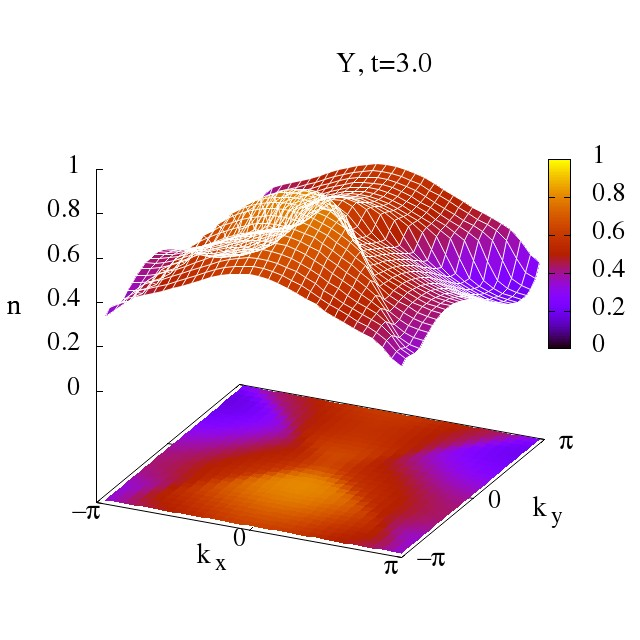
\includegraphics[width=1\linewidth]{figure/y/u3/A_300.jpg}} \\(d)
\end{minipage}
\begin{minipage}[h]{0.43\linewidth}
\center{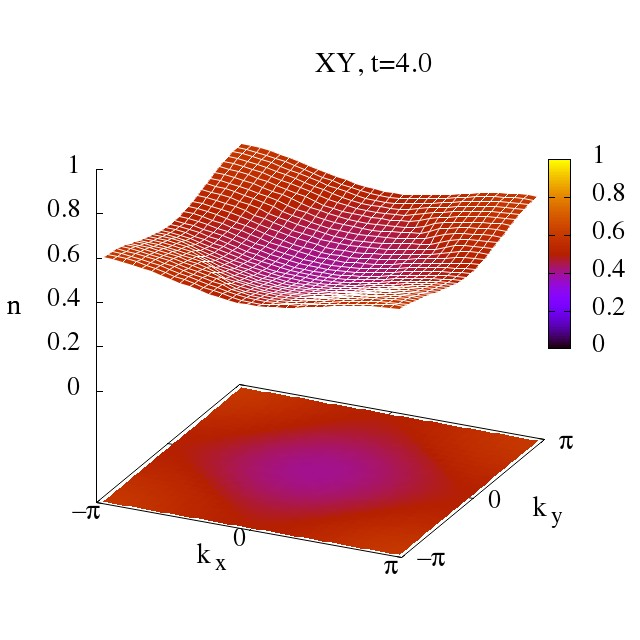
\includegraphics[width=1\linewidth]{figure/xy/u3/A_400.jpg}} (e) \\
\end{minipage}
\hfill
\begin{minipage}[h]{0.43\linewidth}
\center{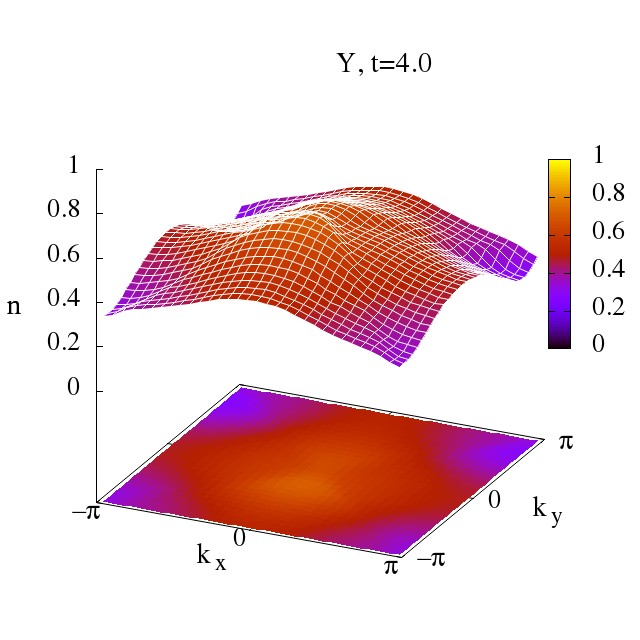
\includegraphics[width=1\linewidth]{figure/y/u3/A_400.jpg}} \\(f)
\end{minipage}
\caption{Momentum distribution for U=3 in different times (from 2 to 4), $\tau$=4. Left column a,c,e - field in XY direction; right column b,d,f - field in Y direction.}
\label{fig:md_u3_A_max}
\end{figure}
%\clearpage


\begin{figure}[h!]
\begin{minipage}[h]{0.43\linewidth}
\center{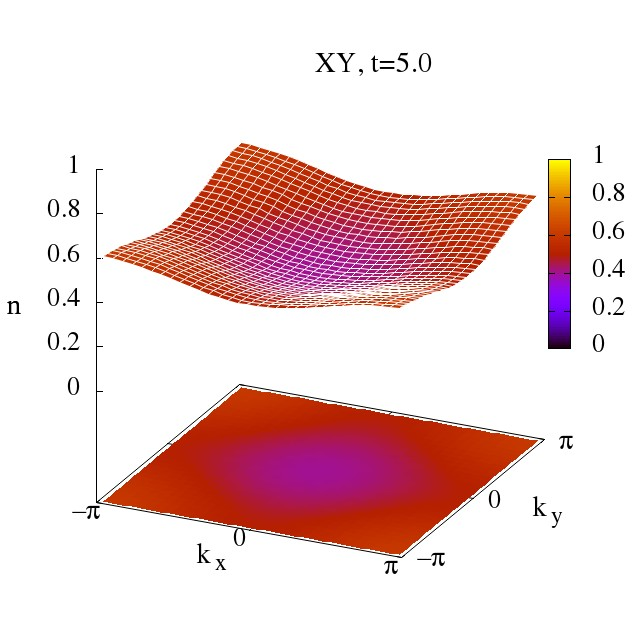
\includegraphics[width=1\linewidth]{figure/xy/u3/A_500.jpg}} (a) \\
\end{minipage}
\hfill
\begin{minipage}[h]{0.43\linewidth}
\center{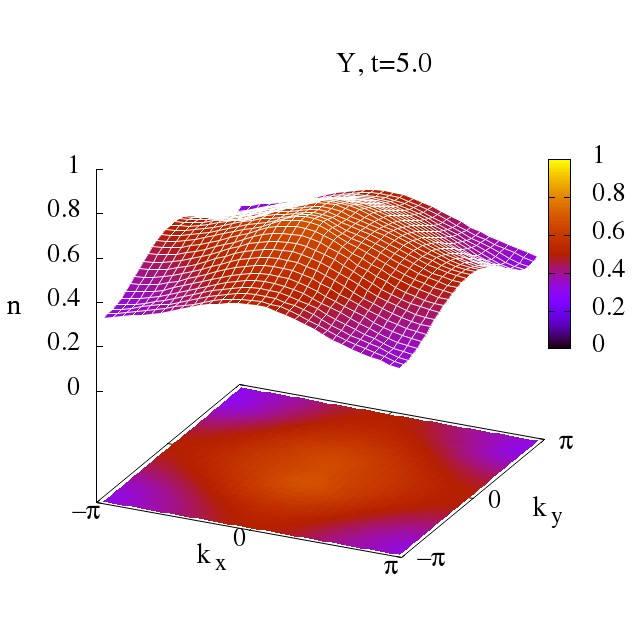
\includegraphics[width=1\linewidth]{figure/y/u3/A_500.jpg}} \\(b)
\end{minipage}
\begin{minipage}[h]{0.43\linewidth}
\center{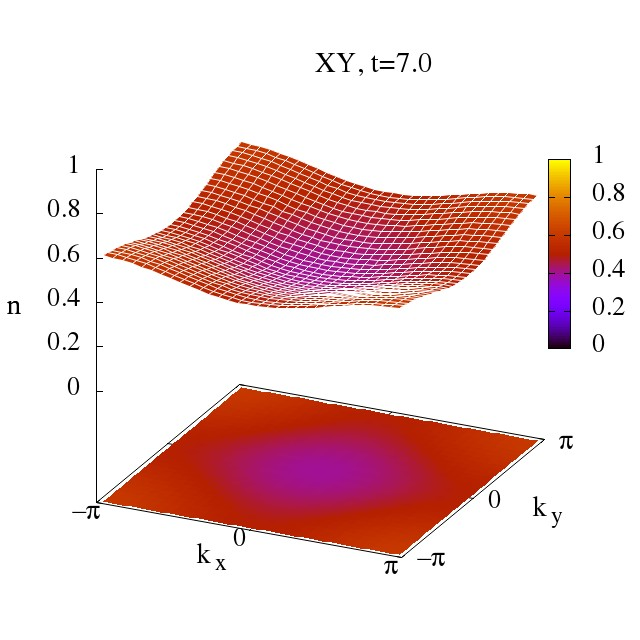
\includegraphics[width=1\linewidth]{figure/xy/u3/A_700.jpg}} (c) \\
\end{minipage}
\hfill
\begin{minipage}[h]{0.43\linewidth}
\center{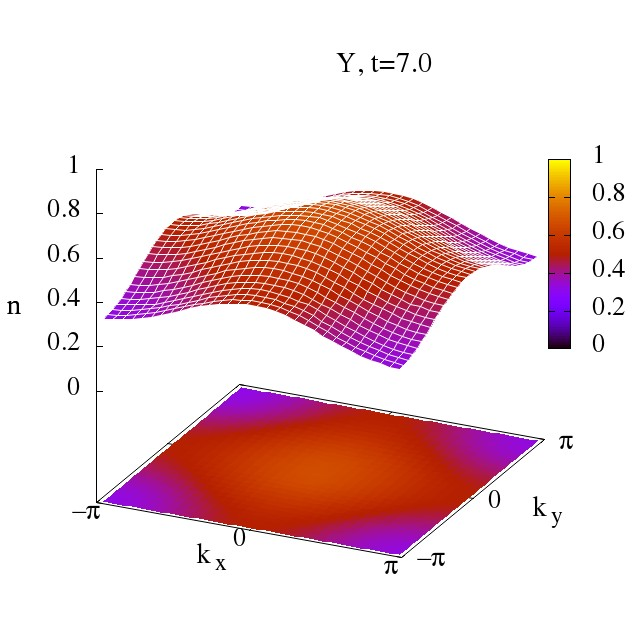
\includegraphics[width=1\linewidth]{figure/y/u3/A_700.jpg}} \\(d)
\end{minipage}
\caption{Relaxation of momentum distribution (after pulse) for U=3 in times 5 and 7, $\tau$=4. Left column a,c - field in XY direction; right column b,d - field in Y direction.}
\label{fig:md_u3_A_max_relaxation}
\end{figure}


In Figure \ref{fig:md_u3_A_max} is shown momentum distribution for U=3 during the action of the pulse. In the diagonal direction of the field (Figure \ref{fig:md_u3_A_max}a,c,e), the shift and flattening of the momentum distribution are seen. This shift leads to inversion of the population. Distribution after exitation does not change (Figures \ref{fig:md_u3_A_max_relaxation}a,c). In Figure \ref{fig:E_tot}a seen that after the pulse the total energy is positive but less than in the case of U=2.

For a field in Y-direction there is no population inversion (Figures \ref{fig:md_u3_A_max}b,d,f). Under the influence of the field, it also shifts to the value of the vector potential. For the Y-direction momentum distribution has a short relaxation time (Figures \ref{fig:md_u3_A_max_relaxation}b,d).

Thus, as the interaction is increased so that the momentum distribution becomes flatter for all directions. This can be associated not only with correlation effects which together with the electric field change the topology of the momentum distribution, but also with an increase in the effective temperature of the system.

Increasing the value of the Coulomb interaction reduces the relaxation time of the distribution after radiation. This is clearly seen in comparing the results of relaxation for the Y direction of the field for different values of the interaction.
\clearpage

\subsubsection{Momentum distribution. $0.8A_{max}$-pulse.}


\begin{figure}[h!]
\begin{minipage}[h]{0.43\linewidth}
\center{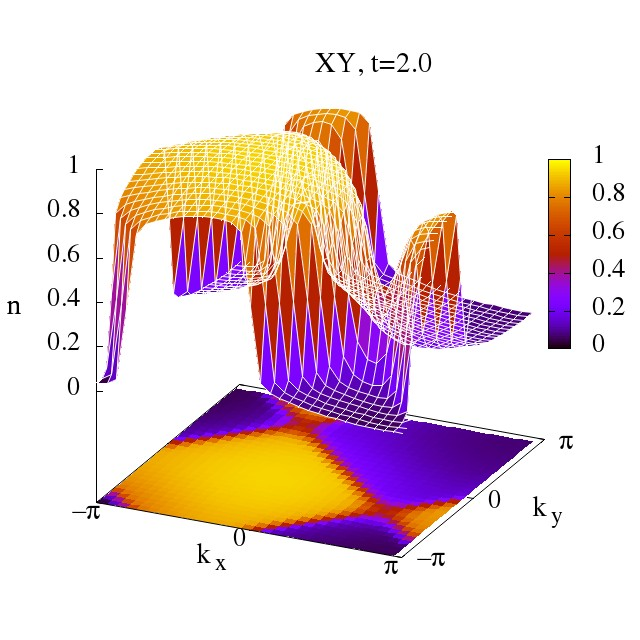
\includegraphics[width=1\linewidth]{figure/xy/u2_08A/A_200.jpg}} (a) \\
\end{minipage}
\hfill
\begin{minipage}[h]{0.43\linewidth}
\center{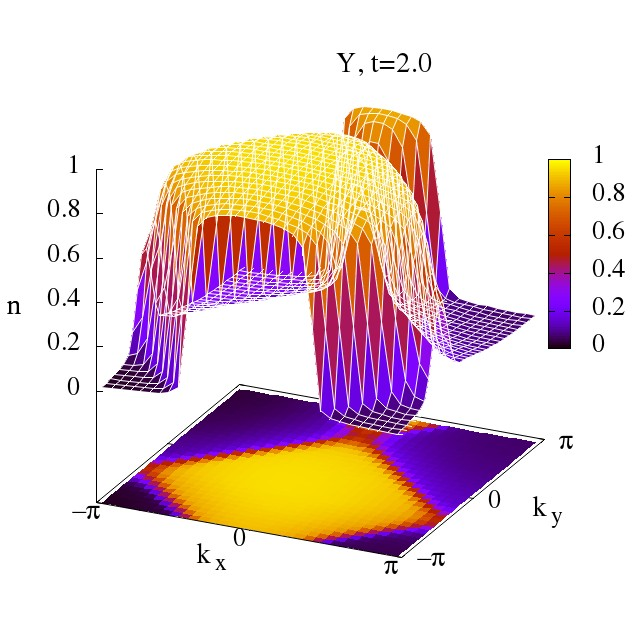
\includegraphics[width=1\linewidth]{figure/y/u2_08A/A_200.jpg}} \\(b)
\end{minipage}
\begin{minipage}[h]{0.43\linewidth}
\center{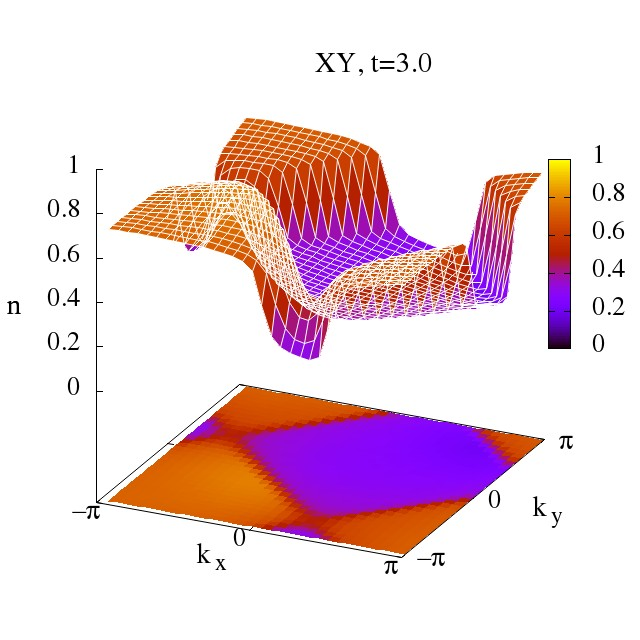
\includegraphics[width=1\linewidth]{figure/xy/u2_08A/A_300.jpg}} (c) \\
\end{minipage}
\hfill
\begin{minipage}[h]{0.43\linewidth}
\center{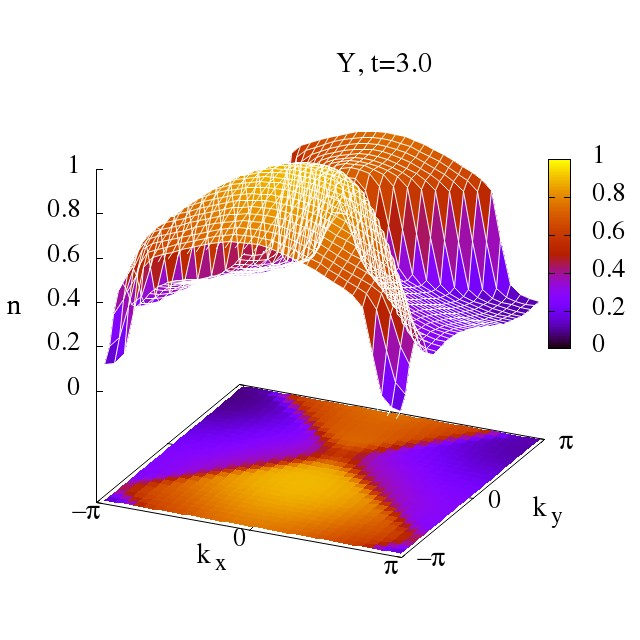
\includegraphics[width=1\linewidth]{figure/y/u2_08A/A_300.jpg}} \\(d)
\end{minipage}
\begin{minipage}[h]{0.43\linewidth}
\center{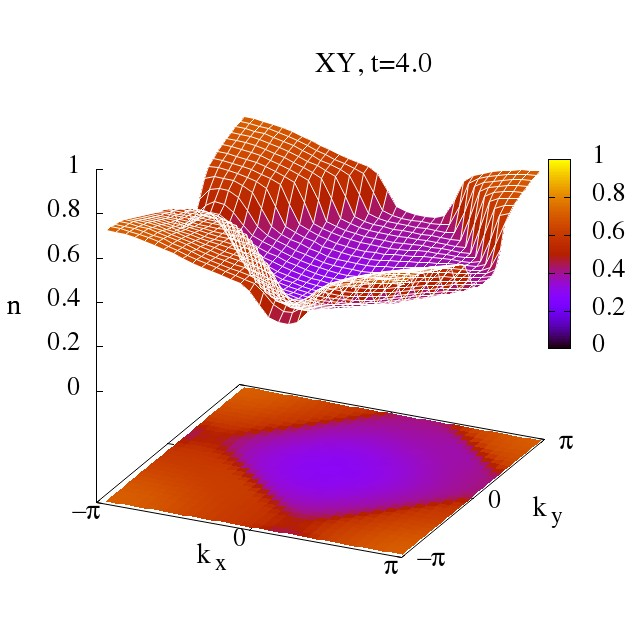
\includegraphics[width=1\linewidth]{figure/xy/u2_08A/A_400.jpg}} (e) \\
\end{minipage}
\hfill
\begin{minipage}[h]{0.43\linewidth}
\center{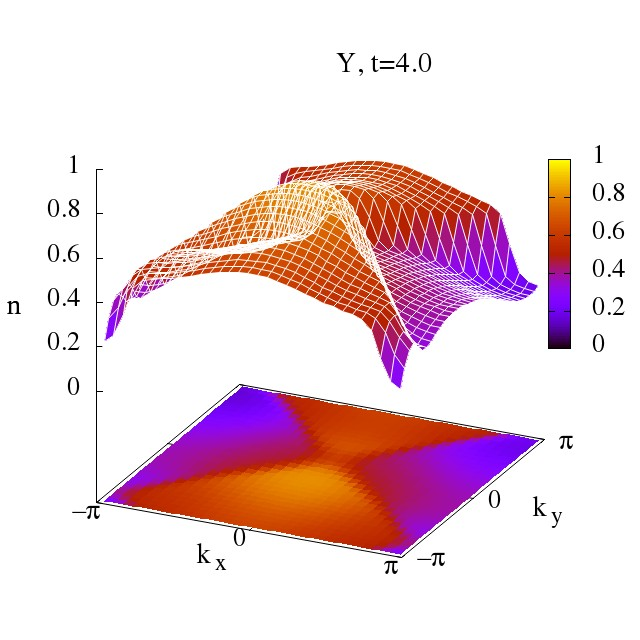
\includegraphics[width=1\linewidth]{figure/y/u2_08A/A_400.jpg}} \\(f)
\end{minipage}
\caption{Momentum distribution for U=2 in different times (from 2 to 4), $\tau$=4. Left column a,c,e - field in XY direction; right column b,d,f - field in Y direction.}
\label{fig:md_u2_08A}
\end{figure}
%\clearpage


\begin{figure}[h!]
\begin{minipage}[h]{0.43\linewidth}
\center{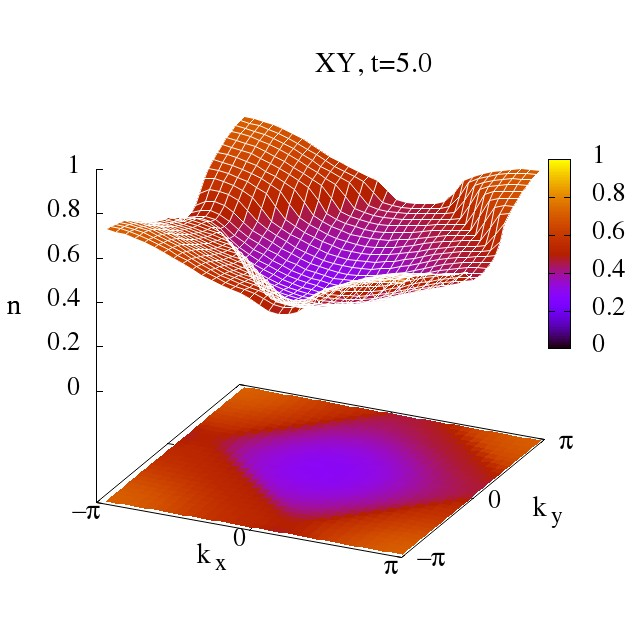
\includegraphics[width=1\linewidth]{figure/xy/u2_08A/A_500.jpg}} (a) \\
\end{minipage}
\hfill
\begin{minipage}[h]{0.43\linewidth}
\center{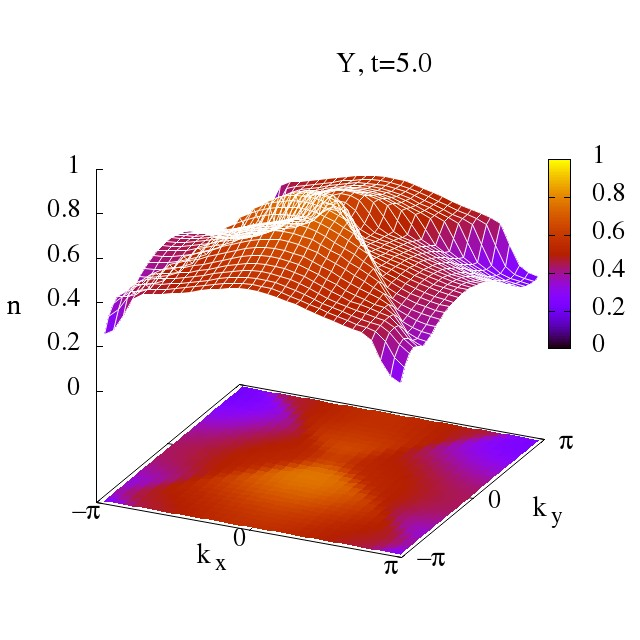
\includegraphics[width=1\linewidth]{figure/y/u2_08A/A_500.jpg}} \\(b)
\end{minipage}
\begin{minipage}[h]{0.43\linewidth}
\center{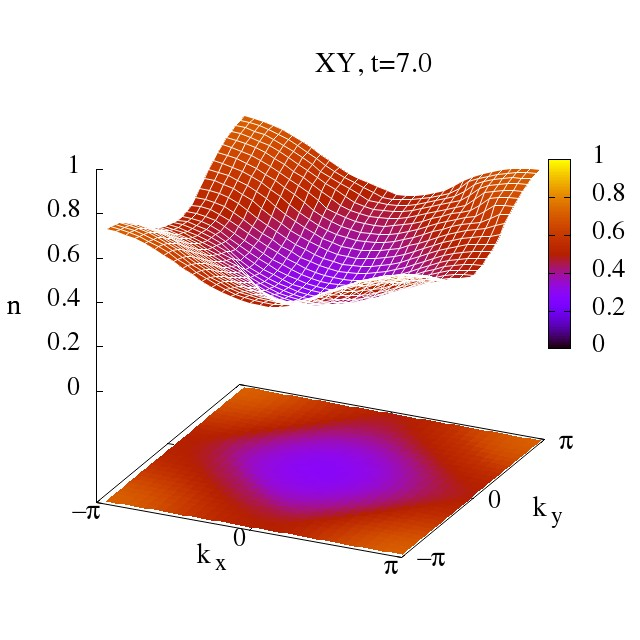
\includegraphics[width=1\linewidth]{figure/xy/u2_08A/A_700.jpg}} (c) \\
\end{minipage}
\hfill
\begin{minipage}[h]{0.43\linewidth}
\center{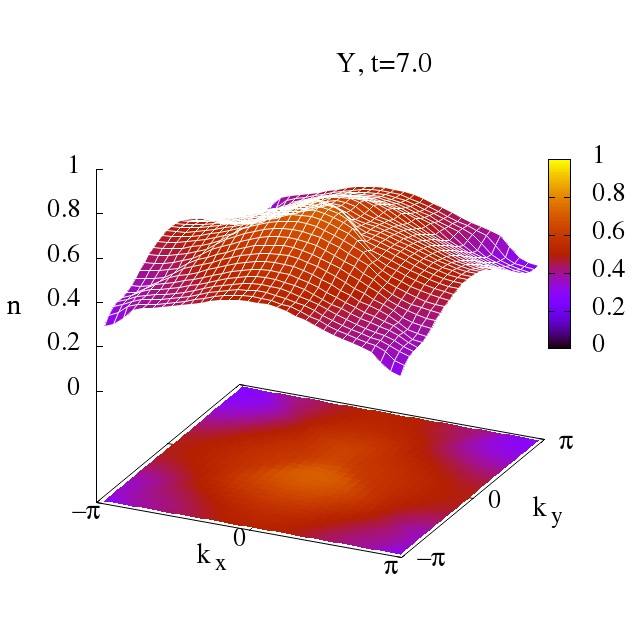
\includegraphics[width=1\linewidth]{figure/y/u2_08A/A_700.jpg}} \\(d)
\end{minipage}
\begin{minipage}[h]{0.43\linewidth}
\center{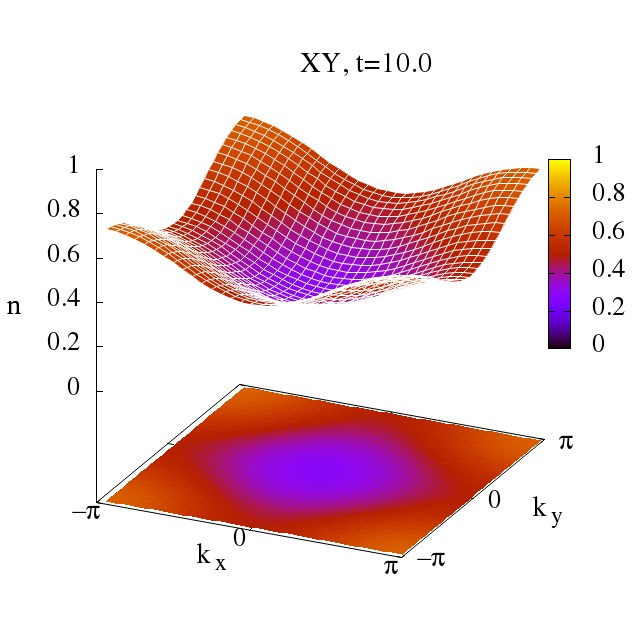
\includegraphics[width=1\linewidth]{figure/xy/u2_08A/A_1000.jpg}} (e) \\
\end{minipage}
\hfill
\begin{minipage}[h]{0.43\linewidth}
\center{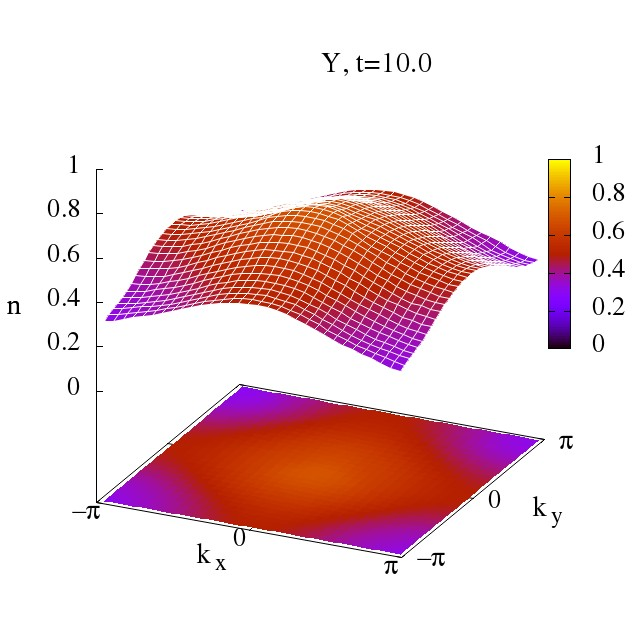
\includegraphics[width=1\linewidth]{figure/y/u2_08A/A_1000.jpg}} \\(f)
\end{minipage}
\caption{Relaxation of momentum distribution (after pulse) for U=2 in different times (from 5 to 10), $\tau$=4. Left column a,c,e - field in XY direction; right column b,d,f - field in Y direction.}
\label{fig:md_u2_08A_relaxation}
\end{figure}

In Figures \ref{fig:md_u2_08A} and \ref{fig:md_u2_08A_relaxation} is shown momentum distribution for U=2 during the action of the pulse and relaxation. There were used a pulses with $0.8A_{max}$. This do not allows to shift the momentum distribution in the case of Y-field from $\Gamma$ to Y during excitation, in the case of diagonal field from $\Gamma$ to M in the Brillouin zone during the pulse. This can be seen in the Figures \ref{fig:md_u2_08A}e,f, these are the graphs of the momentum distribution in which the pulse end.

In the process of relaxation Figures \ref{fig:md_u2_08A_relaxation}a,c,e, the minimum of the momentum distribution shifted to the $\Gamma$ point for diagonal field. It take place because the system needs to adjust the momentum shift to $\pi\sqrt{2}$ to achieve a thermal state. The distribution relax to thermal states with $T_{eff} < 0$.
As expected, field in Y direction does not turn over distribution of electrons (Figure \ref{fig:md_u2_08A_relaxation}b,d,f). Effect of shifting to the $\Gamma$ point of maximum population exist to reach a thermal state.


Geometry of 2D square lattice give us possibility to investigate polarization dependence of physical quantity. Due to this, the behavior of the system under the action of a linearly polarized fields in the diagonal and Y direction was considered.

In the case of a diagonal field, many effects have been found which in agreement with the article \citet{PhysRevB.85.155124} such as population inversion, behaviour of relaxation of the momentum distribution to the thermal state in case of non optimal vector potential. 

For Y field direction population inversion is not observed at the considered parameters of the laser pulse and the Coulomb interaction. This is seen in the graphs of the total energy, double occupancy and the momentum distribution. Distribution has a long relaxation time compared with the results for the diagonal field direction. 

It is important to note how the parameters of the system and the pulse separately affect the distribution. In equilibrium, correlations and temperature blur Fermi step, the electric field used as a vector potential simply shifts the distribution by the value of this vector potential. In nonequilibrium in the absence of correlations, the momentum distribution moves in the direction of the vector potential without changing its shape. 
A common effect in both directions of the field is the distortion of the momentum distribution under the action of the combined effects of correlations, the electric field and an increase of the effective temperature.

\subsection{Change the sign of the interaction using a circularly polarized field}


We continue investigate situation when system has change of sign of interaction. In this part we focused in behaviour of the single-band Hubbard model under circularly polarized vector potentials on a 2D square lattice. 

Selecting the parameters of a pulse possible to change of the interaction from repulsive to attractive by different scenarios. As noted earlier, the most popular way to change the population in this section will be transferring the middle point of the momentum distribution, which is located in the $\Gamma$ point of the first Brillouin zone initially before pulse, to the M point. For this purpose we use a half- mono- and multi-cycle pulses with different shape and phase parameters. 


\subsubsection{Polarization dependence of the circular $\pi$-pulse}

Consider the transition from linear to circular polarization for half-cycle pulse. Figure \ref{fig:Pulses_3} shows the graphs of vector potentials. Pulse parameters are written in the Table  \ref{table:3}. 

\begin{table}[h!]
\begin{center}
  \begin{tabular}{ | c | c | c | c | c |}
    \hline
    $A$ & $\omega$ & $FWHM$ & $\phi_x$ & $\phi_y$ \\ \hline
    -4.44 & 1.0 & 1.0 & $3\pi /4$ & $\pi /4$  \\ \hline
    -3.625 & 1.0 & 1.0 & $2\pi /3$ & $\pi /3$   \\ \hline
    -3.25 & 1.0 & 1.0 & $7\pi /12$ & $5\pi /12$   \\ \hline
    -3.14 & 1.0 & 1.0 & $\pi /2$ & $\pi /2$   \\    
    \hline
  \end{tabular}
\caption{Pulse parameters}
\label{table:3}
\end{center}
\end{table}

\begin{figure}[h!]
\begin{minipage}[h]{0.5\linewidth}
\center{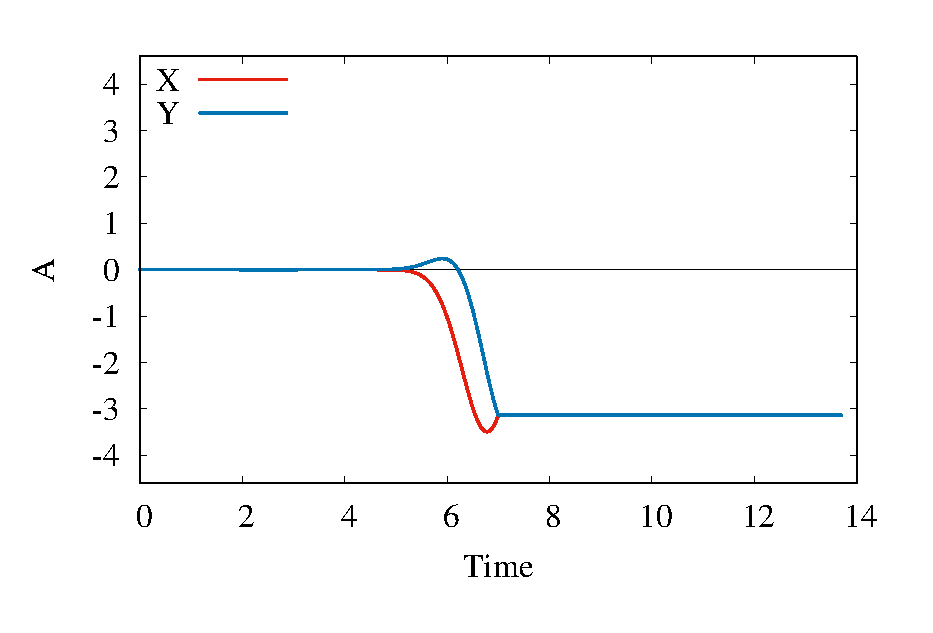
\includegraphics[width=1\linewidth]{figure_c/3/Pulse_1.eps}} (a) \\
\end{minipage}
\hfill
\begin{minipage}[h]{0.5\linewidth}
\center{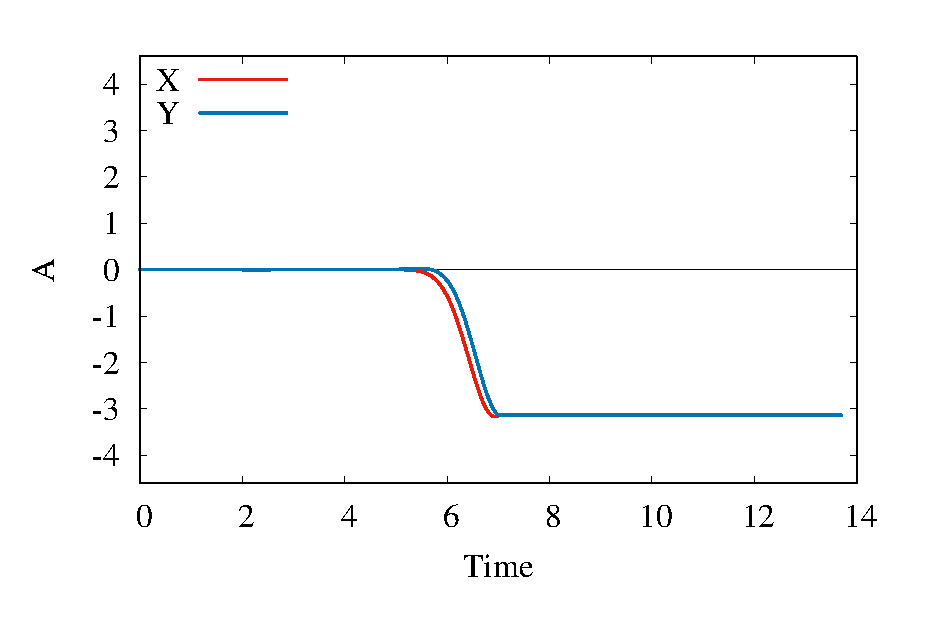
\includegraphics[width=1\linewidth]{figure_c/3/Pulse_3.eps}} \\(c)
\end{minipage}
\begin{minipage}[h]{0.5\linewidth}
\center{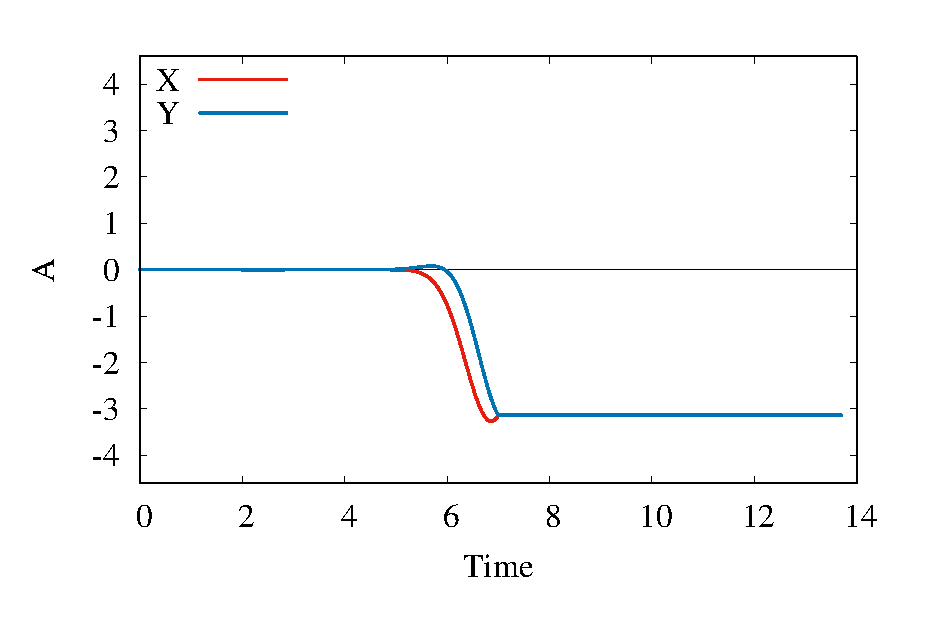
\includegraphics[width=1\linewidth]{figure_c/3/Pulse_2.eps}} (b) \\
\end{minipage}
\hfill
\begin{minipage}[h]{0.5\linewidth}
\center{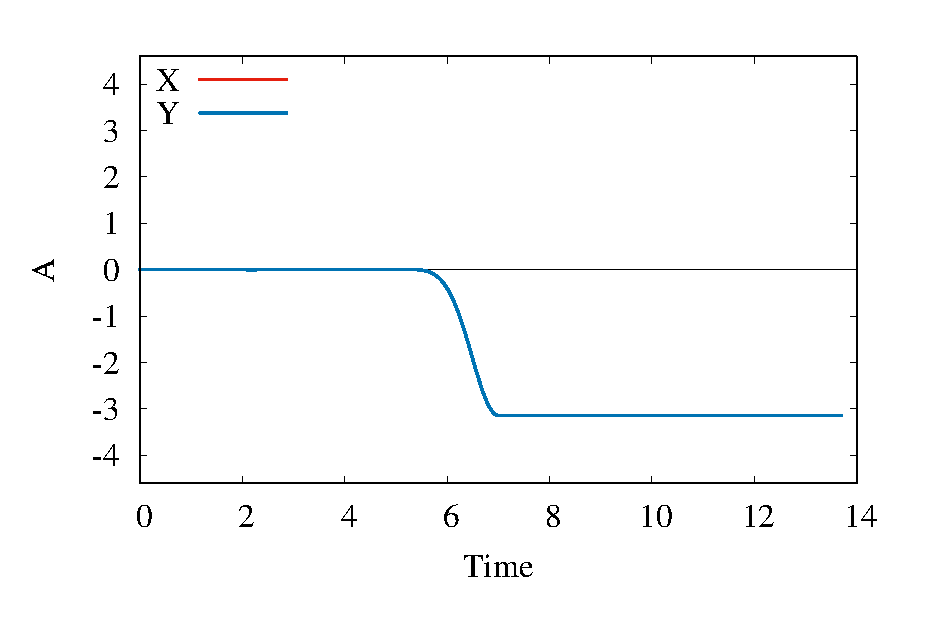
\includegraphics[width=1\linewidth]{figure_c/3/Pulse_4.eps}} \\(d)
\end{minipage}
\caption{Vector potentials.}
\label{fig:Pulses_3}
\end{figure}


The trajectory of the center of momentum distribution is shown in Figure \ref{fig:Pulse_p_3}. As we can see, this trajectory strongly depends on the polarization and the amplitude of the vector potential. The curves with an initial phase equal to $\phi_y=\pi /4$ corresponds to circular polarization, $\phi_y=\pi /3$ and $\phi_y=5\pi /12$ are elliptical and $\phi_y=\pi /2$ has linear polarization.

For calculations used monocycle condition as:

\begin{equation}
FWHM={1 \over \omega}\\
\label{eq:monocycle_condition}
\end{equation}

were FWHM - full width at half maximum, $\omega$ - frequency.

\begin{figure}[h!]
\center{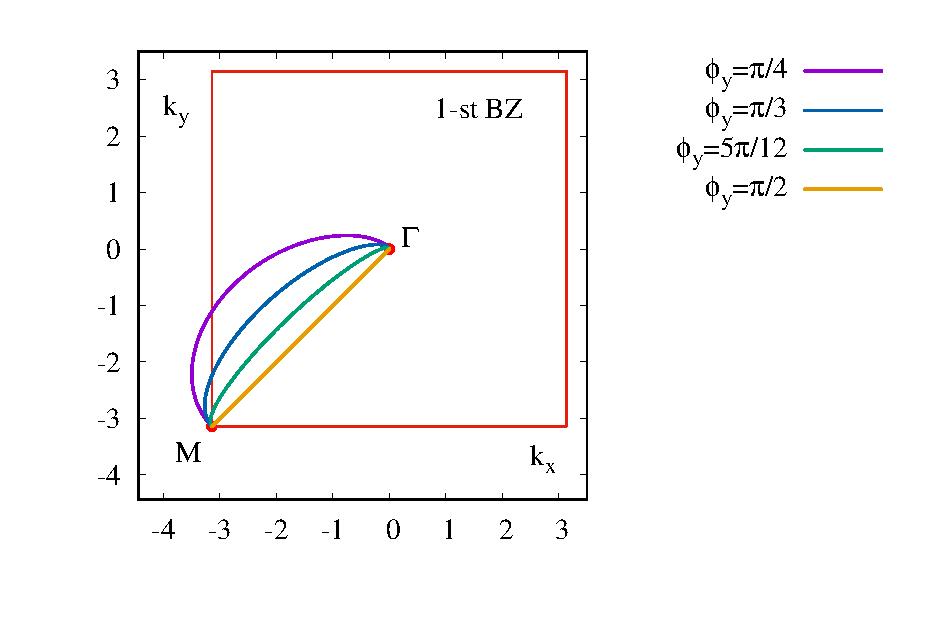
\includegraphics[width=0.7\linewidth]{figure_c/3/Pulse_p.eps}} \\
\caption{Middle point trajectories of the momentum distribution.}
\label{fig:Pulse_p_3}
\end{figure}

 
\begin{figure}[h!]
\begin{minipage}[h]{0.5\linewidth}
\center{\includegraphics[width=1\linewidth]{figure_c/3/Etot.eps}} (a) \\
\end{minipage}
\hfill
\begin{minipage}[h]{0.5\linewidth}
\center{\includegraphics[width=1\linewidth]{figure_c/3/docc.eps}} \\(b)
\end{minipage}
\caption{Total energy and double occupancy.}
\label{fig:Etot_3}
\end{figure}


To obtain a larger population inversion, it better to apply the pulse with linear polarization; this can be seen from the graph of total energy in Figure \ref{fig:Etot_3}a. With a gradual increase in polarization from linear to circular, the final value of the total energy decreases slightly. But double occupancy (Figure \ref{fig:Etot_3}b) almost does not depend on the phase between the X and Y components of the field.

\clearpage


\subsubsection{The frequency dependence of the circular $\pi$-pulse}

Now we look at how the physical parameters of the model change under the action of half-cycle circularly polarized vector potentials with different frequencies. Figure \ref{fig:Pulses_2} shows the graphs vector potentials for this cases. 


\begin{figure}[h!]
\begin{minipage}[h]{0.5\linewidth}
\center{\includegraphics[width=1\linewidth]{figure_c/2/Pulse_0.eps}} (a) \\
\end{minipage}
\hfill
\begin{minipage}[h]{0.5\linewidth}
\center{\includegraphics[width=1\linewidth]{figure_c/2/Pulse_3.eps}} \\(d)
\end{minipage}
\begin{minipage}[h]{0.5\linewidth}
\center{\includegraphics[width=1\linewidth]{figure_c/2/Pulse_1.eps}} (b) \\
\end{minipage}
\hfill
\begin{minipage}[h]{0.5\linewidth}
\center{\includegraphics[width=1\linewidth]{figure_c/2/Pulse_4.eps}} \\(e)
\end{minipage}
\begin{minipage}[h]{0.5\linewidth}
\center{\includegraphics[width=1\linewidth]{figure_c/2/Pulse_2.eps}} (c) \\
\end{minipage}
\hfill
\begin{minipage}[h]{0.5\linewidth}
\center{\includegraphics[width=1\linewidth]{figure_c/2/Pulse_5.eps}} \\(f)
\end{minipage}
\caption{Vector potentials.}
\label{fig:Pulses_2}
\end{figure}

Pulse parameters are written in the Table \ref{table:2}. 

\begin{table}[h!]
\begin{center}
  \begin{tabular}{ | c | c | c | c | c |}
    \hline
    $A$ & $\omega$ & $FWHM$ & $\phi_x$ & $\phi_y$ \\ \hline
    -4.44 & 0.25 & 4.0 & $3\pi /4$ & $\pi /4$  \\ \hline
    -4.44 & 0.5 & 2.0 & $3\pi /4$ & $\pi /4$   \\ \hline
    -4.44 & 1.0 & 1.0 & $3\pi /4$ & $\pi /4$   \\ \hline
    -4.44 & 1.5 & 0.667 & $3\pi /4$ & $\pi /4$   \\ \hline
    -4.44 & 2.0 & 0.5 & $3\pi /4$ & $\pi /4$   \\ \hline
    -4.44 & 16.0 & 0.0625 & $3\pi /4$ & $\pi /4$   \\ 

    \hline
  \end{tabular}
\caption{Pulse parameters}
\label{table:2}
\end{center}
\end{table}

As shown in Figure \ref{fig:Pulse_p_2}, the trajectory of the momentum distribution is the same everywhere. But the frequencies are different, which means the higher the frequency, the faster the momentum distribution will move from the $\Gamma$ point of the Brillouin zone to M. 

Total energy and double occupancy responds strongly to such a frequency change. In Figure \ref{fig:Etot_2} it can be seen that the higher the frequency of the pulse, the greater the total energy and double population, and therefore the greater the population inversion.

\begin{figure}[h!]
\center{\includegraphics[width=0.7\linewidth]{figure_c/2/Pulse_p.eps}} \\
\caption{Middle point trajectories of the momentum distribution.}
\label{fig:Pulse_p_2}
\end{figure}


\begin{figure}[h!]
\begin{minipage}[h]{0.5\linewidth}
\center{\includegraphics[width=1\linewidth]{figure_c/2/Etot.eps}} (a) \\
\end{minipage}
\hfill
\begin{minipage}[h]{0.5\linewidth}
\center{\includegraphics[width=1\linewidth]{figure_c/2/docc.eps}} \\(b)
\end{minipage}
\caption{Total energy and double occupancy.}
\label{fig:Etot_2}
\end{figure}

As example, in Figure \ref{fig:md_2} depicted the behavior of the momentum distribution in the circular field at different points in time for $U=2$. The shape of the vector potential for the figure \ref{fig:md_2} corresponds to figure \ref{fig:Pulses_2}c.   Distribution graphs move in the direction of the vector potential at $Time=$5.0 to $Time=$7.0 because electric field switched on (Figures \ref{fig:md_2}a-d). After $Time=$7.0 proses of relaxation start, distribution stop moving and until $Time=$10.0 topology become more smoother.


\begin{figure}[h!]
\begin{minipage}[h]{0.43\linewidth}
\center{\includegraphics[width=1\linewidth]{figure_c/2/A_550.jpg}} (a) \\
\end{minipage}
\hfill
\begin{minipage}[h]{0.43\linewidth}
\center{\includegraphics[width=1\linewidth]{figure_c/2/A_700.jpg}} \\(d)
\end{minipage}
\begin{minipage}[h]{0.43\linewidth}
\center{\includegraphics[width=1\linewidth]{figure_c/2/A_600.jpg}} (b) \\
\end{minipage}
\hfill
\begin{minipage}[h]{0.43\linewidth}
\center{\includegraphics[width=1\linewidth]{figure_c/2/A_750.jpg}} \\(e)
\end{minipage}
\begin{minipage}[h]{0.43\linewidth}
\center{\includegraphics[width=1\linewidth]{figure_c/2/A_650.jpg}} (c) \\
\end{minipage}
\hfill
\begin{minipage}[h]{0.43\linewidth}
\center{\includegraphics[width=1\linewidth]{figure_c/2/A_1000.jpg}} \\(f)
\end{minipage}
\caption{Momentum distribution for pulse with $\omega$=1, FWHM=1.}
\label{fig:md_2}
\end{figure}

\clearpage





\subsubsection{Circular monocycle pulse with different initial phases.}

Let us proceed to consider how the properties of the Hubbard model change under the influence of monosycle pulses taken at different values of the initial phase (Figure \ref{fig:Pulses_1}).

\begin{figure}[h!]
\begin{minipage}[h]{0.5\linewidth}
\center{\includegraphics[width=1\linewidth]{figure_c/1/u_0/Pulse_1.eps}} (a) \\
\end{minipage}
\hfill
\begin{minipage}[h]{0.5\linewidth}
\center{\includegraphics[width=1\linewidth]{figure_c/1/u_0/Pulse_3.eps}} \\(c)
\end{minipage}
\begin{minipage}[h]{0.5\linewidth}
\center{\includegraphics[width=1\linewidth]{figure_c/1/u_0/Pulse_2.eps}} (b) \\
\end{minipage}
\hfill
\begin{minipage}[h]{0.5\linewidth}
\center{\includegraphics[width=1\linewidth]{figure_c/1/u_0/Pulse_4.eps}} \\(d)
\end{minipage}
\caption{Vector potentials.}
\label{fig:Pulses_1}
\end{figure}

Pulse parameters are written in the Table \ref{table:1}. Phase for the vector potential in Y-direction taken as initial. 

Moving the maximum of the momentum distribution, which was originally located at the $\Gamma$ point of the Brillouin zone to the M point as depicted in the Figure \ref{fig:Pulse_p_1}. 


\begin{table}[h!]
\begin{center}
  \begin{tabular}{ | c | c | c | c | c |}
    \hline
    $A$ & $\omega$ & $FWHM$ & $\phi_x$ & $\phi_y$ \\ \hline
    -4.44 & 1.0 & 1.0 & $\pi /2$ & 0  \\ \hline
    -4.44 & 1.0 & 1.0 & $2\pi /3$ & $\pi /6$   \\ \hline
    -4.44 & 1.0 & 1.0 & $3\pi /4$ & $\pi /4$   \\ \hline
    -4.44 & 1.0 & 1.0 & $5\pi /6$ & $\pi /3$   \\    
    \hline
  \end{tabular}
\caption{Pulse parameters}
\label{table:1}
\end{center}
\end{table}

The Figure \ref{fig:Etot_1} shows the total energy and double occupancy for different values of the initial phases of the vector potential and for various Coulomb interactions. Figure \ref{fig:Etot_1}a depicts the total energy for a pulse at zero Coulomb interaction. The maximum value of the total energy is reached for $\phi_y=\pi /4$. Total energys for $\phi_y=\pi /6$ and $\phi_y=\pi /3$ are symmetrical relative to the middle of the  pulse ($t=7$) and graph for $\phi_y=0$ symmetrical itself since it is always equidistant from M points of the Brillouin zone during the whole pulse time (Figure \ref{fig:Pulse_p_1} red line). Double occupancy (Figure \ref{fig:Etot_1}a) is equal $0.25$ during all time, which must be in case of $U=0$.



\begin{figure}[h!]
\center{\includegraphics[width=0.7\linewidth]{figure_c/1/u_0/Pulse_p.eps}} \\
\caption{Middle point trajectories of the momentum distribution.}
\label{fig:Pulse_p_1}
\end{figure}


Depending on the magnitude of interaction, symmetry with respect to the middle of the pulse disappears gradually. Figures \ref{fig:Etot_1}a and \ref{fig:Etot_1}b show the total energy and double occupancy for a monocycle pulse at different initial phases in the case of $U=2$. All the considered pulses in one way or another lead to population inversion. Total energys for $\phi_y=\pi /6$ and $\phi_y=\pi /3$ are not any more symmetrical relative to the middle of pulse $t=7$. Curve at $\phi_y=\pi /6$ has bigger maximum of total energy compare to $\phi_y=\pi /3$. It seems that increasing the interaction increases the absorption of energy by the system and thus increases the temperature during a pulse. The temperature rise makes a flatter momentum distribution that reduces the value of the population inversion, because more electrons are now may extend to the edges of "hat" of the momentum distribution. At the same time, as shown by previous calculations, the form of the “hat” of the momentum distribution for a correlated system itself may vary during the pulse. Thus, competition of the effects: the inclusion of correlations that tend to bend the "hat" of the momentum distribution, shifting the momentum distribution by the vector potential to a more favorable position and heating the system, may explain why we see the maximum value of the total energy and double occupancy for the pulse with $\phi_y=\pi /3$ slightly larger than for $\phi_y=\pi /4$ in Figure \ref{fig:Etot_1}b,d.



 


\clearpage

\begin{figure}[h!]
\begin{minipage}[h]{0.5\linewidth}
\center{\includegraphics[width=1\linewidth]{figure_c/1/u_0/Etot.eps}} (a) \\
\end{minipage}
\hfill
\begin{minipage}[h]{0.5\linewidth}
\center{\includegraphics[width=1\linewidth]{figure_c/1/u_0/docc.eps}} \\(c)
\end{minipage}
\begin{minipage}[h]{0.5\linewidth}
\center{\includegraphics[width=1\linewidth]{figure_c/1/u_2/Etot.eps}} (b) \\
\end{minipage}
\hfill
\begin{minipage}[h]{0.5\linewidth}
\center{\includegraphics[width=1\linewidth]{figure_c/1/u_2/docc.eps}} \\(d)
\end{minipage}
\caption{Total energy and double occupancy.}
\label{fig:Etot_1}
\end{figure}

\clearpage



\subsubsection{Away from monocycle condition for $\pi$-pulse.}


\begin{figure}[h!]
\begin{minipage}[h]{0.5\linewidth}
\center{\includegraphics[width=1\linewidth]{figure_c/4/Pulse_1.eps}} (a) \\
\end{minipage}
\hfill
\begin{minipage}[h]{0.5\linewidth}
\center{\includegraphics[width=1\linewidth]{figure_c/4/Pulse_3.eps}} \\(c)
\end{minipage}
\begin{minipage}[h]{0.5\linewidth}
\center{\includegraphics[width=1\linewidth]{figure_c/4/Pulse_2.eps}} (b) \\
\end{minipage}
\hfill
\begin{minipage}[h]{0.5\linewidth}
\center{\includegraphics[width=1\linewidth]{figure_c/4/Pulse_4.eps}} \\(d)
\end{minipage}
\caption{Vector potentials.}
\label{fig:Pulses_4}
\end{figure}

Figure \ref{fig:Pulses_4} shows the graphs of half-cycle circularly polarized vector potentials with different ratios FWHM and $\omega$. The monocycle condition chousen as in Formula \ref{furmula:mc} and depicted for half-cycle pulse in Figure \ref{fig:Pulses_4}a. Pulse parameters are written in the Table \ref{table:4}. By increasing the frequency of pulse and leaving the FWHM constant, we move away from the monosicle condition. This is clearly seen on the Figure \ref{fig:Pulse_p_4} of the trajectory of center of the momentum distribution for $\pi$-pulse.

\begin{table}[h!]
\begin{center}
  \begin{tabular}{ | c | c | c | c | c |}
    \hline
    $A$ & $\omega$ & $FWHM$ & $\phi_x$ & $\phi_y$ \\ \hline
    -4.44 & 1.0 & 1.0 & $3\pi /4$ & $\pi /4$  \\ \hline
    -4.44 & 2.0 & 1.0 & $3\pi /4$ & $\pi /4$   \\ \hline
    -4.44 & 3.0 & 1.0 & $3\pi /4$ & $\pi /4$   \\ \hline
    -4.44 & 4.0 & 1.0 & $3\pi /4$ & $\pi /4$   \\    
    \hline
  \end{tabular}
\caption{Pulse parameters}
\label{table:4}
\end{center}
\end{table}


\begin{figure}[h!]
\center{\includegraphics[width=0.7\linewidth]{figure_c/4/Pulse_p.eps}} \\
\caption{Middle point trajectories of the momentum distribution.}
\label{fig:Pulse_p_4}
\end{figure}

The total energy of such pulses (Figure \ref{fig:Etot_4}) has a different structure during the pulse, nevertheless optimal inversion presented the $\pi$-pulse with monocycle condition. This can be explained by the fact that $\pi$-pulse with monocycle condition have the shortest way to move the center of the momentum distribution from $\Gamma$ to M point, which contributes to less heating of the system. The appearance of a peak at the total energy that crosses the zero value at $t \sim 6.2$ is due to the fact that the center of the momentum distribution in the case of non-monocycle passes near another M point in the first Brillouin zone, thereby creating an inversion on that part of the trajectory.


\begin{figure}[h!]
\begin{minipage}[h]{0.5\linewidth}
\center{\includegraphics[width=1\linewidth]{figure_c/4/Etot.eps}} (a) \\
\end{minipage}
\hfill
\begin{minipage}[h]{0.5\linewidth}
\center{\includegraphics[width=1\linewidth]{figure_c/4/docc.eps}} \\(d)
\end{minipage}
\caption{Total energy and double occupancy.}
\label{fig:Etot_4}
\end{figure}

\clearpage




\subsubsection{Multicycle pulse.}

In this part, we discuss how to create a maximum population inversion during multicycle circularly polarized pulse. Vector potential depicted in Figure \ref{fig:Pulses_5} has a ramp at the beginning and end, the rest of the pulse has the same amplitude. The maximum amplitude of the vector potential is 4.44.


For this purpose, pulse was chosen that move the middle of the momentum distribution through all four M points in the 2d square lattice Brillouin zone (Figure \ref{fig:Pulse_p_5}).






\begin{figure}[h!]
\begin{minipage}[h]{0.5\linewidth}
\center{\includegraphics[width=1\linewidth]{figure_c/plot/Pulse_1.eps}} (a) \\
\end{minipage}
\hfill
\begin{minipage}[h]{0.5\linewidth}
\center{\includegraphics[width=1\linewidth]{figure_c/plot/Pulse_3.eps}} \\(c)
\end{minipage}
\begin{minipage}[h]{0.5\linewidth}
\center{\includegraphics[width=1\linewidth]{figure_c/plot/Pulse_2.eps}} (b) \\
\end{minipage}
\hfill
\begin{minipage}[h]{0.5\linewidth}
\center{\includegraphics[width=1\linewidth]{figure_c/plot/Pulse_4.eps}} \\(d)
\end{minipage}
\caption{Vector potentials.}
\label{fig:Pulses_5}
\end{figure}

\clearpage


\begin{figure}[h!]
\begin{minipage}[h]{0.5\linewidth}
\center{\includegraphics[width=1\linewidth]{figure_c/plot/Pulse_p_w1.eps}} (a) \\
\end{minipage}
\hfill
\begin{minipage}[h]{0.5\linewidth}
\center{\includegraphics[width=1\linewidth]{figure_c/plot/Pulse_p_w6.eps}} \\(c)
\end{minipage}
\begin{minipage}[h]{0.5\linewidth}
\center{\includegraphics[width=1\linewidth]{figure_c/plot/Pulse_p_w3.eps}} (b) \\
\end{minipage}
\hfill
\begin{minipage}[h]{0.5\linewidth}
\center{\includegraphics[width=1\linewidth]{figure_c/plot/Pulse_p_w12.eps}} \\(d)
\end{minipage}
\caption{Middle point trajectories of the momentum distribution.}
\label{fig:Pulse_p_5}
\end{figure}

The total energy (Figure \ref{fig:Etot_5}) shows that the main part of the curve is in the positive area of the graph during the pulse. Double occupancy tend to go above 0.25. All this facts indicates that the system during the pulse most of the time has different sign of the interaction in comparison with the equilibrium solution.

\clearpage

\begin{figure}[h!]

\begin{minipage}[h]{0.5\linewidth}
\center{\includegraphics[width=1\linewidth]{figure_c/plot/Etot_1.eps}} (a) \\
\end{minipage}
\hfill
\begin{minipage}[h]{0.5\linewidth}
\center{\includegraphics[width=1\linewidth]{figure_c/plot/docc_1.eps}} \\(e)
\end{minipage}

\begin{minipage}[h]{0.5\linewidth}
\center{\includegraphics[width=1\linewidth]{figure_c/plot/Etot_2.eps}} (b) \\
\end{minipage}
\hfill
\begin{minipage}[h]{0.5\linewidth}
\center{\includegraphics[width=1\linewidth]{figure_c/plot/docc_2.eps}} \\(f)
\end{minipage}

\begin{minipage}[h]{0.5\linewidth}
\center{\includegraphics[width=1\linewidth]{figure_c/plot/Etot_3.eps}} (c) \\
\end{minipage}
\hfill
\begin{minipage}[h]{0.5\linewidth}
\center{\includegraphics[width=1\linewidth]{figure_c/plot/docc_3.eps}} \\(g)
\end{minipage}

\begin{minipage}[h]{0.5\linewidth}
\center{\includegraphics[width=1\linewidth]{figure_c/plot/Etot_4.eps}} (d) \\
\end{minipage}
\hfill
\begin{minipage}[h]{0.5\linewidth}
\center{\includegraphics[width=1\linewidth]{figure_c/plot/docc_4.eps}} \\(h)
\end{minipage}


\caption{Total energy and double occupancy.}
\label{fig:Etot_5}
\end{figure}

\clearpage



1. With a circular vector potential, the maximum positive value of the total energy depends on the initial phase. To create maximum of population inversion, it is not necessary to have a phase due to which the middle of momentum distribution is transferred exactly from the $\Gamma$ point to M, this case is shown in the Figure \ref{fig:Etot_1}b.

2. The higher the frequency, the greater the population inversion creates the circulary polarized $\pi$-pulse (Figure \ref{fig:Etot_2}).

3. Creating of the population inversion becomes more efficient in linear $\pi$-pulse compare to circularly polarized $\pi$-pulse (Figure \ref{fig:Etot_3}a).

4. It is possible to create several peaks with positive total energy during half-oscillation or more of vector potential (Figure \ref{fig:Etot_4}a).

To create a population inversion more than once we need to adjust: amplitude of the vector potential, which sets the magnitude of the oscillations and the pulse should be more than a monocycle (Figure \ref{fig:Pulses_5}). Thus, if one adjust the shape of the vector potential, is possible to achieve an pulse that moves the middle point of the momentum distribution from the $\Gamma$ point through (or close) all four M points of the first Brillouin zone (Figure \ref{fig:Pulse_p_5}).
